\documentclass[12pt]{article}
\usepackage{graphicx}
\usepackage{amsthm}
\usepackage{amsmath}
\usepackage{amssymb}
\usepackage{microtype}
\usepackage{array}
\usepackage{booktabs}
\usepackage{longtable}

\usepackage[left=3cm,right=1.5cm,top=2.5cm,bottom=2.5cm]{geometry}

% Allow a little extra stretch on hard-to-break lines (long \texttt names, wide
% inline math) to avoid small overfull boxes.
\setlength{\emergencystretch}{2em}

\usepackage{setspace}
\onehalfspacing

\usepackage{fontspec}
\IfFontExistsTF{Sylfaen}{
  \newfontfamily{\titlepagefont}{Sylfaen}[AutoFakeBold=1.0]
}{
  \newfontfamily{\titlepagefont}{Liberation Serif}
}
\setmainfont{Times New Roman}

% Monospaced font for Rocq listings: Consolas covers most of the Unicode symbols
% used verbatim in the Coq sources; a fallback supplies any it lacks (e.g. emptyset).
\newfontfamily{\rocqfont}{Consolas}

\usepackage{listings}
\lstdefinestyle{thesiscode}{
  basicstyle=\ttfamily\small,
  columns=fullflexible,
  keepspaces=true,
  showstringspaces=false,
  frame=single,
  numbers=left,
  numbersep=8pt,
  xleftmargin=1em,
  xrightmargin=1em,
  aboveskip=0.75\baselineskip,
  belowskip=0.75\baselineskip,
  breaklines=true
}

% Listing style for Rocq/Coq source, used in the formalisation section.
\lstdefinelanguage{Rocq}{
  morekeywords={Module,Import,Export,Inductive,Definition,Fixpoint,Record,
    Theorem,Lemma,Proof,Qed,Defined,match,with,end,if,is,then,else,fun,
    forall,exists,Type,Prop,bool,Set,Variable,Hypothesis,Section,return,let,in,
    From,Require,Notation},
  sensitive=true,
  morecomment=[s]{(*}{*)},
  morestring=[b]"
}
\lstdefinestyle{rocqstyle}{
  language=Rocq,
  basicstyle=\rocqfont\footnotesize,
  keywordstyle=\bfseries,
  commentstyle=\itshape,
  columns=fullflexible,
  keepspaces=true,
  showstringspaces=false,
  frame=single,
  numbers=left,
  numbersep=8pt,
  xleftmargin=1.2em,
  xrightmargin=0.5em,
  aboveskip=0.75\baselineskip,
  belowskip=0.75\baselineskip,
  breaklines=true,
  extendedchars=true,
  inputencoding=utf8
}

\usepackage[style=ieee,backend=biber,sorting=nyt]{biblatex}
\addbibresource{references.bib}

\usepackage{tikz}
\usetikzlibrary{arrows.meta,positioning,automata}
\usepackage{placeins}

\usepackage[hidelinks]{hyperref}


\newcommand{\cR}{{\mathcal R}}
\def\cut{\mu}
\def\eg{{\em e.g.\ }}
\def\ie{{\em i.e.\ }}
\newtheorem{definition}{Definition}[section]
\newtheorem{proposition}{Proposition}[section]
\newtheorem{lemma}{Lemma}[section]
\newtheorem{theorem}{Theorem}[section]
\newtheorem{remark}{Remark}[section]
\newtheorem{conjecture}{Conjecture}[section]


\newcommand{\thesisUniversity}{Kutaisi International University}
\newcommand{\thesisSchool}{School of Computer Science}
\newcommand{\thesisProgram}{Bachelor's Program in Computer Science}
\newcommand{\thesisStudentName}{Mariam Katamashvili}
\newcommand{\thesisTitle}{Formalization of Crisp and Fuzzy Derivatives of Regular Expressions in Rocq}
\newcommand{\thesisDegree}{Bachelor of Computer Science}
\newcommand{\thesisSupervisorName}{Besik Dundua}
\newcommand{\thesisSupervisorPosition}{Professor}
\newcommand{\thesisSecondSupervisorName}{Furio Honsell}
\newcommand{\thesisSecondSupervisorPosition}{Professor}
\newcommand{\thesisPlaceYear}{Kutaisi, 2026}

\begin{document}

\hypersetup{pageanchor=false}
\begin{titlepage}
\thispagestyle{empty}
\begingroup
\singlespacing
\begin{center}
{\titlepagefont\bfseries\fontsize{14}{17}\selectfont
\thesisUniversity\\
\thesisSchool\\
\thesisProgram\par}

\vspace{2cm}

{\titlepagefont\bfseries\fontsize{16}{19}\selectfont
\thesisStudentName\par}

\vspace{2cm}

{\titlepagefont\bfseries\fontsize{16}{19}\selectfont
\thesisTitle\par}

\vspace{3cm}

{\titlepagefont\fontsize{14}{17}\selectfont
The thesis is completed for obtaining the academic degree of\\
\thesisDegree\par}

\vspace{3cm}

{\titlepagefont\fontsize{12}{15}\selectfont
\thesisSupervisorName\par}

\vspace{1cm}

{\titlepagefont\fontsize{12}{15}\selectfont
\thesisSupervisorPosition\par}

\vspace{1.5cm}

{\titlepagefont\fontsize{12}{15}\selectfont
\thesisSecondSupervisorName\par}

\vspace{1cm}

{\titlepagefont\fontsize{12}{15}\selectfont
\thesisSecondSupervisorPosition\par}

\vfill

{\titlepagefont\fontsize{12}{15}\selectfont
\thesisPlaceYear\par}
\end{center}
\endgroup
\end{titlepage}
\clearpage

\hypersetup{pageanchor=true}

\pagenumbering{roman}
\section*{Declaration}
\addcontentsline{toc}{section}{Declaration}

I, the author of this bachelor's thesis, declare that the thesis is my own original work
and does not contain any material previously published, submitted for publication, or
presented for defense by other authors, unless properly referenced or cited in
accordance with academic standards.

\vspace{2cm}

\noindent \thesisStudentName

\vspace{1cm}

\noindent \today

\clearpage

\section*{Abstract}
\addcontentsline{toc}{section}{Abstract}

This thesis studies Brzozowski derivatives of regular expressions in two settings,
the classical crisp one and a fuzzy one based on similarity, and verifies the theorems
in the Rocq proof assistant. In the crisp setting it defines derivatives of regular languages and expressions, the
correspondence between the syntactic and the semantic derivative, the finiteness of
the set of derivatives, and the construction of the deterministic automaton that has
canonical derivatives as its states. The original contribution is the fuzzy layer,
which replaces exact symbol matching by a similarity relation cut at a threshold
$\mu$. Its main observation is that, under the minimum triangular norm,
cut-similarity is an equivalence relation. A fuzzy derivative over the alphabet is
then just an ordinary derivative over the quotient alphabet obtained by identifying
similar symbols. Through this quotient construction regularity, the
semantic-syntactic correspondence, finiteness, and correctness of the fuzzy
automaton all carry over from the crisp theory. The automaton recognises exactly
the words that lie within threshold $\mu$ of some word of the original language.
The claims are checked by a proof assistant rather than argued only on paper.

\bigskip
\noindent\textbf{Keywords:} regular expressions, Brzozowski derivatives, finite
automata, fuzzy similarity, triangular norms, formal verification, Rocq.

\clearpage


\setcounter{tocdepth}{2}
\tableofcontents
\clearpage

\pagenumbering{arabic}

\section{Introduction}\label{sec:introduction}

Regular expressions were introduced by Stephen Kleene in the 1950s~\cite{Kleene1956}
as a notation for describing the patterns that a finite-state machine can recognise. The idea was to
capture, with a few simple operators for union, concatenation and Kleene star,
exactly the languages accepted by finite automata. That correspondence between a 
piece of syntax and a machine has proved to be one of the most durable ideas
in computer science. Regular expressions are interesting precisely because they sit
at this meeting point of theory and practice. On the theoretical side they describe a
well-understood class of languages and come with a rich algebra. On the practical
side they are
everywhere, from the lexical analysers inside every compiler, through search and
text processing, to validation of input and scanning of network traffic. A notation
that a programmer types in seconds is backed by decades of automata theory, and that
is what makes getting its foundations right worthwhile.

The common way to run a regular expression is to compile it into a finite automaton
and then let the machine consume the input, using one of the classical
constructions of Thompson~\cite{Thompson1968}, Glushkov~\cite{Glushkov1962}, or
McNaughton and Yamada~\cite{McNaughtonYamada1960}. There is also an older and more
direct idea, due to Brzozowski~\cite{B64}, that this thesis takes as its starting
point. Rather than building a separate machine, one can differentiate the expression
itself: the derivative of an expression with respect to a symbol describes what
remains to be matched after that symbol has been consumed, so iterating it across an
input word is already a way of running the expression. When derivatives are kept in
a canonical form there are only finitely many of them, and taking those canonical
derivatives as states yields a deterministic automaton with no auxiliary
construction at all. The approach has aged well and was reexamined from a modern
implementation perspective by Owens, Reppy and Turon~\cite{OwensReppyTuron}.

Exact matching, however, is often stricter than an application really wants. Text is
noisy, symbols are mistyped or substituted, and two inputs that a person would treat
as the same can differ in a handful of places. This is why fuzziness is interesting:
a great deal of real matching is approximate, and a theory that insists on equality
of symbols cannot describe it. A natural way to relax the rigidity is to replace
equality between symbols by a notion of similarity, so that two symbols match
not only when they are identical but also when they are close enough. Closeness is
measured by a value in $[0,1]$ and combined using triangular norms 
of fuzzy logic~\cite{met05}. The same idea appears in similarity-based logic
programming~\cite{Sessa2002}, where unification is replaced by matching up to a
similarity relation. This thesis asks what becomes of Brzozowski's derivative 
theory once symbols match by similarity. If the consumed symbol only has to be 
similar to the first symbol of a word, up to a threshold $\mu$, does the
derivative-based theory of regular languages and automata still hold together?

It does, for a simple reason.
When similarity is combined with the minimum triangular norm, cutting the similarity
relation at a threshold $\mu$ gives an equivalence relation. A fuzzy derivative over
the alphabet is then just an ordinary derivative over the quotient alphabet, where
symbols similar within $\mu$ are identified. The crisp theory transfers to the fuzzy
setting through this quotient construction. Regularity, the correspondence between
the syntactic and the semantic derivative, finiteness of the set of derivatives, and
correctness of the derivative automaton all carry over. The fuzzy automaton accepts
exactly the words that lie within tolerance $\mu$ of some word of the language.

Derivative and finiteness arguments are easy to get subtly wrong. A proof assistant
checks every step mechanically. The crisp theory is ergo mechanised in the Rocq proof
assistant~\cite{Rocq}, building on the Coquand--Siles formalisation of
regular-expression equivalence via Brzozowski
derivatives~\cite{CoquandRegexEquality,RocqRegexpBrzozowski}. It covers
regular-expression syntax and semantics, nullability, canonicalisation, the
derivative correspondence and automaton correctness, and the similarity
infrastructure on which the fuzzy layer rests. The full development is available in
a repository~\cite{OurRocqRepo}, with the code presented next to the
mathematics it verifies.

The rest of the thesis is organised as follows. Section~\ref{sec:literature} reviews
the existing literature on regular expressions, derivatives, their formalisation, and
fuzzy automata.
Section~\ref{sec:methodology} contains the technical development in two layers: the
crisp theory of derivatives and the derivative automaton, presented together with
its Rocq formalisation, followed by the fuzzy layer with its definitions, the
quotient construction, and the fuzzy automaton. Section~\ref{sec:conclusion}
summarises the results.

\section{Literature Review}\label{sec:literature}

The theory this thesis builds on splits into a few strands that have largely
developed in parallel, and it is worth seeing where each of them stands before
combining them. The first strand is the classical correspondence between regular
expressions and finite automata. The standard constructions that realise an
expression as a machine are Thompson's translation into a nondeterministic automaton
with epsilon transitions~\cite{Thompson1968}, the position automaton of
Glushkov~\cite{Glushkov1962}, and the state-graph method of McNaughton and
Yamada~\cite{McNaughtonYamada1960}. These remain the textbook routes from syntax to
machine, and they treat the automaton as an object to be built alongside the
expression rather than read off from it.

A second strand reasons about regular expressions algebraically. Conway's account of
regular algebra and finite machines~\cite{C71} organises the equational theory,
while Salomaa gave complete axiom systems for the algebra of regular
events~\cite{Salomaa} and Kozen later established completeness for Kleene algebra
and the algebra of regular events~\cite{Kozen}. This line is concerned with when two
expressions denote the same language and with axiomatising that equivalence, which
is a different question from how to match efficiently, but it is closely related,
since deciding equivalence is one of the things a good normal form for expressions
should help with.

The derivative approach sits between these two and is the one this thesis takes as
its starting point. Brzozowski introduced derivatives of regular
expressions~\cite{B62} and showed that differentiating an expression with respect to
a symbol, together with a test for whether the empty word is accepted, is enough to
both decide membership and construct a deterministic automaton, provided expressions
are identified up to a few simplifications so that only finitely many derivatives
arise. Owens, Reppy and Turon re-examined the construction from a modern
implementation perspective~\cite{OwensReppyTuron} and showed that it remains both
elegant and practical, particularly because it extends smoothly to intersection and
complement. Derivatives are attractive precisely because the automaton is latent in
the expression rather than assembled separately, which is also what makes the method
a good fit for mechanised reasoning.

That fit has been borne out by work on formalising regular languages in proof
assistants. The development this thesis extends descends from the Coquand--Siles
decision procedure for regular-expression equivalence in type
theory~\cite{CoquandRegexEquality} and its accompanying Rocq
formalisation of Brzozowski derivatives~\cite{RocqRegexpBrzozowski}, carried out in
the Rocq proof assistant~\cite{Rocq}. Mechanising this material forces every
simplification and every finiteness argument to be made explicit, which is exactly
where paper proofs tend to be informal, and it is the foundation on which the
similarity layer of the present work is added.

The fuzzy side of the picture has its own substantial literature, though it has
mostly grown from a different root. The dominant tradition equips automata and
expressions with membership values rather than crisp acceptance, so that a word is
recognised to a degree. Li and Pedrycz studied fuzzy finite automata and fuzzy
regular expressions with membership values in lattice-ordered
monoids~\cite{LP06}, Stamenkovi\'c and \'Ciri\'c gave constructions of fuzzy automata
from fuzzy regular expressions~\cite{SC12}, and Garhwal, Jiwari and Tomasiello
surveyed fuzzy regular languages and fuzzy automata more broadly~\cite{GJT17}. A
related quantitative and coalgebraic perspective appears in the quantitative Kleene
coalgebras of Silva, Bonchi, Bonsangue and Rutten~\cite{SilvaBonchiBonsangueRutten2011}
and, more recently, in the extension of the quantitative pattern-matching paradigm by
Alves, Kesner and Ramos~\cite{AlvesKesnerRamos2025}. The technical backdrop for all
of this is the theory of triangular norms and fuzzy logic, of which Metcalfe's notes
give a compact account~\cite{met05}.

What is distinctive about the route taken here is the source of the fuzziness. Rather
than attaching weights to transitions or to acceptance, this thesis keeps acceptance
crisp and instead loosens the matching of symbols, so that a symbol matches any other
symbol that is similar to it within a chosen threshold. This is the same move that
Sessa made in approximate logic programming, where unification is replaced by
matching up to a similarity relation~\cite{Sessa2002}, transposed from resolution to
derivatives. The payoff is that, under the minimum T-norm, the fuzzy theory reduces
to the crisp one over a quotient alphabet, which keeps the derivative machinery and
its formalisation intact instead of requiring a separate weighted theory. The
present work therefore connects the derivative-based and formally verified treatment
of regular expressions with the similarity-based style of approximate matching, and
the membership-value tradition cited above is the natural point of comparison for
what such a similarity-based account does and does not capture.

\section{Methodology and Results}\label{sec:methodology}

Rocq (until
recently called Coq) is an interactive proof assistant built on a constructive
dependent type theory, the Calculus of Inductive
Constructions~\cite{CoquandHuet1988,CoqArt}, a descendant of Martin-L\"of's
intuitionistic type theory~\cite{MartinLof1984}. What makes such a system able to
check mathematics is the \emph{propositions-as-types} principle, also known as the
Curry--Howard correspondence~\cite{Howard1980}. A proposition is read as a type, and
a proof of that proposition is read as a \emph{term} (a program) whose type is
exactly that proposition. Proving a statement therefore means constructing an object of the
corresponding type, and a statement is regarded as true precisely when its type is
inhabited.

Under this reading the logical connectives become the type-forming operations of a
functional programming language, so that proofs are literally functional programs.
A proof of an implication $A \Rightarrow B$ is a function that turns any proof of
$A$ into a proof of $B$; a proof of a conjunction $A \wedge B$ is a pair holding a
proof of each conjunct; a proof of a disjunction $A \vee B$ is a tagged value that
records which side holds together with a proof of it; a proof of a universal
statement $\forall x.\,P(x)$ is a (dependent) function mapping each $x$ to a proof
of $P(x)$; and a proof of an existential statement $\exists x.\,P(x)$ is a
(dependent) pair consisting of a witness $a$ together with a proof of $P(a)$. This
is the \emph{proofs-as-programs} paradigm. Because proofs are programs, they can be
run, and the computation steps of the type theory correspond to the simplification
of proofs. 

Both paradigms depend on the logic being \emph{constructive}
(intuitionistic) rather than classical. In
intuitionistic logic a proof of $\exists x.\,P(x)$ must exhibit a witness,
and a proof of $A \vee B$ must say which disjunct holds. This is what makes
the corresponding proof terms carry the data a program needs in order to compute,
namely the witness and the chosen branch. Classical logic abandons that discipline.
Its principles, the law of excluded middle $A \vee \neg A$ and
double-negation elimination $\neg\neg A \Rightarrow A$, are not theorems of
intuitionistic logic. A classical proof of an existential need not produce any
witness. One may prove that an object exists by deriving a contradiction from
its non-existence, without ever naming it. Such a proof has no computational
content, and there is no program to extract from it. Were Rocq founded on classical
rather than intuitionistic logic, the propositions-as-types reading would survive
only as a formal analogy. Proofs would no longer be programs that can be run. The
witnesses and decision procedures this thesis relies on could not be obtained from
the proofs that justify them, and the executable character of the formalisation
would be lost. The constructive foundation is ergo not an incidental choice. It
is what makes the formalised theory compute. (Classical axioms can be
added to Rocq consistently when needed, but doing so reintroduces
this loss of computational content, and the development does not use them.)

In practice one rarely writes these proof terms by hand, because for any nontrivial
statement the term is large. Instead Rocq is driven by \emph{tactics}, commands
that build the proof term indirectly, working backwards from the goal. At each point
the system displays a \emph{proof state} consisting of the hypotheses
available and the goal still to be proved. Each tactic transforms that state,
reducing the goal or splitting it into subgoals while assembling
the corresponding fragment of the proof term. The tactics mirror the
type-theoretic operations described above. For instance \texttt{intro} moves the
premise of an implication into the hypotheses (introducing a function abstraction),
\texttt{apply} uses an implication or lemma to reduce the goal to its premises
(function application, \ie\ modus ponens), and \texttt{induction} invokes the
induction principle of an inductive datatype. When every subgoal has been
discharged, the command \texttt{Qed} submits the finished term to Rocq's
kernel, which type-checks it independently. The tactics are only a
way of producing the term. It is the kernel's check, not the tactic
script, that is believed. The Rocq listings shown in this section are the
statements and definitions from this process. The tactic
scripts that prove them are available in the repository~\cite{OurRocqRepo}.

\subsection{Preliminaries}\label{sec:prelim}

\begin{definition}[Alphabet, words, and languages]
\mbox{}\\[-0.5em]
\begin{itemize}
    \item An \emph{alphabet} $\Sigma$ is a finite, nonempty set of symbols.
    \item A \emph{word} over $\Sigma$ is a finite sequence of symbols from $\Sigma$.
    \item The \emph{empty word} is denoted by $\varepsilon$.
    \item The \emph{set of all words} over $\Sigma$ is $\Sigma^*$.
    \item A \emph{language} over $\Sigma$ is a subset $\mathcal{L} \subseteq \Sigma^*$.
\end{itemize}
\end{definition}

In Rocq the alphabet is abstract, given by the module type \texttt{SYM}, which
fixes a type \texttt{A} of symbols with decidable equality (an \texttt{eqType}). A
word is then a finite list of symbols, \texttt{seq A}, with the empty word written
\texttt{[::]}, and a language is a boolean predicate on words, \texttt{pred word},
so that membership is a decidable test.

\begin{lstlisting}[style=rocqstyle,caption={Alphabet, words, and languages (\texttt{Alphabet.v}, \texttt{Languages.v}).},label={lst:words}]
(* A plain alphabet of symbols. This is the minimal interface needed for
   words, languages, regular-expression syntax, and semantics. *)
Module Type SYM.
  Parameter A : eqType.
End SYM.

(* A word over the alphabet A is a finite sequence of symbols from A.
   The empty word ε is written directly as [::]. *)
Definition word := seq A.

(* A language over A is a decidable predicate on words. *)
Definition language := pred word.
\end{lstlisting}

\begin{definition}[Regular expressions]
The \emph{regular expressions}, or \emph{regular events}, over an alphabet
$\Sigma$, written $E^{\Sigma}$, are defined by the grammar
\[
  r ::= \emptyset \mid \varepsilon \mid a\ (a \in \Sigma)
        \mid r+r \mid r\cdot r \mid r^* \mid r \,\&\, r \mid \neg r,
\]
where $a$ ranges over $\Sigma$. The intended meanings are: $\emptyset$ the empty
language; $\varepsilon$ the language $\{\varepsilon\}$; $a$ the singleton $\{a\}$;
$+$ union; $\cdot$ concatenation; ${}^{*}$ Kleene star; $\&$ intersection; and
$\neg$ complement.
\end{definition}

\begin{definition}[Restricted regular expressions]\label{def:restricted}
The \emph{restricted regular expressions} over $\Sigma$, written $R^{\Sigma}$, are
those regular expressions in which the constructors $\&$ and $\neg$ do not occur;
that is, they are built from $\emptyset$, $\varepsilon$ and the symbols $a\in\Sigma$
using only $+$, $\cdot$ and ${}^{*}$.
\end{definition}

\begin{definition}[Semantic interpretation]
For a regular expression $r$ over $\Sigma$, its \emph{semantic interpretation} is
the language $\mathcal{L}(r) \subseteq \Sigma^*$ defined inductively by
\[
\begin{aligned}
\mathcal{L}(\emptyset)   &= \emptyset, &\qquad
\mathcal{L}(\varepsilon) &= \{\varepsilon\}, \\
\mathcal{L}(a)           &= \{a\},\ a \in \Sigma, &\qquad
\mathcal{L}(r + s)       &= \mathcal{L}(r) \cup \mathcal{L}(s), \\
\mathcal{L}(r \cdot s)   &= \mathcal{L}(r)\cdot\mathcal{L}(s), &\qquad
\mathcal{L}(r^*)         &= \textstyle\bigcup_{n \geq 0} \mathcal{L}(r)^n, \\
\mathcal{L}(r \& s)      &= \mathcal{L}(r) \cap \mathcal{L}(s), &\qquad
\mathcal{L}(\neg r)      &= \Sigma^* \setminus \mathcal{L}(r).
\end{aligned}
\]
\end{definition}

\noindent\textbf{Example.} Over $\Sigma=\{a,b\}$ the expression $(a+b)^{*}\cdot a$
denotes the language of all words that end in $a$, since $(a+b)^{*}$ matches any
prefix and the trailing $a$ fixes the last symbol. It is built only from $+$,
$\cdot$ and ${}^{*}$ and so belongs to the restricted fragment $R^{\Sigma}$. By
contrast $\neg(a\cdot b)$ denotes every word except $ab$, and $a\,\&\,(a+b)$ denotes
$\{a\}$; both use $\neg$ or $\&$ and are ergo not restricted, though still regular.

In Rocq, regular expressions are an inductive datatype whose eight constructors
correspond one-to-one to $\emptyset,\varepsilon,a,+,\cdot,{}^{*},\&,\neg$. The
restricted fragment $R^{\Sigma}$ of Definition~\ref{def:restricted} is carved out
by an inductive predicate \texttt{restricted\_regex}, which holds of an expression
exactly when it is built without \texttt{And} and \texttt{Neg}. The semantic
interpretation $\mathcal{L}(\cdot)$ is the function \texttt{den}, defined by a
structural recursion that maps each constructor to the matching language operation
(\texttt{void}, \texttt{eps}, \texttt{atom}, \texttt{plus}, \texttt{conc},
\texttt{star}, \texttt{prod}, \texttt{compl}).

\begin{lstlisting}[style=rocqstyle,caption={Regular expressions, the restricted fragment, and the semantics (\texttt{RegexSemantics.v}).},label={lst:regex}]
(* Syntax side of semantic interpretation: the regular expressions over A. *)
Inductive regex : Type :=
  | Empty : regex
  | Eps   : regex
  | Char  : A -> regex
  | Alt   : regex -> regex -> regex
  | Seq   : regex -> regex -> regex
  | Star  : regex -> regex
  | And   : regex -> regex -> regex
  | Neg   : regex -> regex.

(* Predicate checking that a regex is restricted, i.e. contains no And or Neg constructors. *)
Inductive restricted_regex : regex -> Prop :=
  | RestrictedEmpty : restricted_regex Empty
  | RestrictedEps   : restricted_regex Eps
  | RestrictedChar  : forall a, restricted_regex (Char a)
  | RestrictedAlt   : forall r s,
      restricted_regex r -> restricted_regex s -> restricted_regex (Alt r s)
  | RestrictedSeq   : forall r s,
      restricted_regex r -> restricted_regex s -> restricted_regex (Seq r s)
  | RestrictedStar  : forall r,
      restricted_regex r -> restricted_regex (Star r).

(* Semantic interpretation: maps each regex to the language it denotes. *)
Fixpoint den (r : regex) : pred word :=
  match r with
  | Empty     => void
  | Eps       => eps
  | Char a    => atom a
  | Alt r1 r2 => plus (den r1) (den r2)
  | Seq r1 r2 => conc (den r1) (den r2)
  | Star r1   => star (den r1)
  | And r1 r2 => prod (den r1) (den r2)
  | Neg r1    => compl (den r1)
  end.
\end{lstlisting}

The language operations that \texttt{den} maps onto are defined in
\texttt{Languages.v}. The empty language, the language of the empty word and the
singleton are immediate. Union, intersection and complement are the pointwise
boolean connectives. Concatenation and Kleene star are decided by a bounded
search over the ways of splitting a word, using helper functions for splitting and
for testing every block of a split.

\begin{lstlisting}[style=rocqstyle,caption={The language operations (\texttt{Languages.v}).},label={lst:langops}]
Definition void : language := pred0.
Definition eps  : language := fun w => w == [::].
Definition atom (a : A) : language := fun w => w == [:: a].

Definition plus (L K : language) : language := fun w => L w || K w.
Definition conc (L K : language) : language :=
  fun w => has (fun i =>
    let u := take i w in
    let v := drop i w in
    L u && K v) (iota 0 (size w).+1).

(* Helpers for Kleene star. *)

(* Checks that every word in sequence belongs to the language.
   This is needed to express membership in the Kleene star. *)
Fixpoint all_in (L : language) (xs : seq word) : bool :=
  match xs with
  | [::] => true
  | x :: xs' => L x && all_in L xs'
  end.

(* Enumerates all finite decompositions of a word into blocks.
   This is the executable counterpart of the union-of-powers view of L*. *)
Fixpoint splits (w : word) : seq (seq word) :=
  match w with
  | [::] => [:: [::] ]
  | a :: w' =>
    flatten [seq
      match ds with
      | [::] => [:: [:: [:: a] ] ]
      | x :: xs => [:: [:: a] :: ds; (a :: x) :: xs]
      end
    | ds <- splits w']
  end.

Definition star (L : language) : language := fun w => has (all_in L) (splits w).
Definition prod (L K : language) : language := fun w => L w && K w.
Definition compl (L : language)  : language := fun w => ~~ L w.
\end{lstlisting}

In many constructions it is useful to know whether the language of an expression
contains the empty word.

\begin{definition}[Nullability]\label{def:nullable}
A regular expression $r$ is \emph{nullable} if $\varepsilon \in \mathcal{L}(r)$. The
\emph{nullable function} $\nu$ is defined by
\[
  \nu(r) =
  \begin{cases}
    \varepsilon & \text{if $r$ is nullable},\\
    \emptyset   & \text{otherwise.}
  \end{cases}
\]
Equivalently, $\nu$ is characterised by the following equations:
\[
\begin{aligned}
     \nu(\emptyset)      &= \emptyset, &\qquad
     \nu(\varepsilon)    &= \varepsilon, \\
     \nu(a)              &= \emptyset,\ a \in \Sigma, &\qquad
     \nu(r+s)            &= \nu(r) + \nu(s), \\
     \nu(r\cdot s)       &= \nu(r)\,\&\,\nu(s), &\qquad
     \nu(r^*)            &= \varepsilon, \\
     \nu(r\,\&\,s)       &= \nu(r)\,\&\,\nu(s), &\qquad
     \nu(\neg r)         &= \varepsilon \text{ if } \nu(r) = \emptyset,
                            \text{ and } \emptyset \text{ if } \nu(r) = \varepsilon.
\end{aligned}
\]
\end{definition}

\noindent\textbf{Example.} The expression $a^{*}$ is nullable, since
$\varepsilon\in\mathcal{L}(a^{*})$, so $\nu(a^{*})=\varepsilon$. The expression
$a\cdot a^{*}$ is not nullable, since every word it denotes has at least one $a$, so
$\nu(a\cdot a^{*})=\emptyset$. For a union the rule gives
$\nu(a+\varepsilon)=\nu(a)+\nu(\varepsilon)=\emptyset+\varepsilon=\varepsilon$.

In the formalisation, nullability is the boolean function \texttt{has\_eps} and
$\nu$ is \texttt{nu}. The lemma
\texttt{nullable\_correct} proves, by induction on the expression, that
\texttt{has\_eps} agrees with semantic membership of the empty word \texttt{[::]}
in the language.

\begin{lstlisting}[style=rocqstyle,escapeinside={(@}{@)},caption={Nullability and its correctness (\texttt{Nullable.v}).},label={lst:nullable}]
(* Boolean test for whether ε belongs to the language of a regex. *)
Fixpoint has_eps (r : regex) : bool :=
  match r with
  | Empty       => false
  | Eps         => true
  | Char _      => false
  | Alt r1 r2   => has_eps r1 || has_eps r2
  | Seq r1 r2   => has_eps r1 && has_eps r2
  | Star _      => true
  | And r1 r2   => has_eps r1 && has_eps r2
  | Neg r1      => ~~ has_eps r1
  end.

Definition nu (r : regex) : regex :=
  if has_eps r then Eps else Empty.

(* The boolean test has_eps r agrees with the semantic definition of nullable [::] \in r. *)
Lemma nullable_correct : forall r, has_eps r = ([::] \in r).
Proof.
  elim=> /=.
  - by [].
  - by [].
  - by move=> a.
  - move=> r1 IH1 r2 IH2; by rewrite IH1 IH2.
  - move=> r1 IH1 r2 IH2.
    rewrite IH1 IH2.
    change (([::] \in r1) && ([::] \in r2) =
            conc (den r1) (den r2) [::]).
    by rewrite /conc (Languages.conc_nil (A:=A) (den r1) (den r2)).
  - move=> r IH.
    have H : star (den r) [::] := Languages.star_nil (A:=A) (den r).
    by case: (star (den r) [::]) H.
  - move=> r1 IH1 r2 IH2; by rewrite IH1 IH2.
  - move=> r IH; by rewrite IH.
Qed.
\end{lstlisting}

The script above and the term below are the same proof in two forms. One is the high level script we write, the other is the low level term Rocq stores and checks. The term makes every induction case and rewrite explicit.

\lstinputlisting[style=rocqstyle,caption={Proof term produced by the script for \texttt{nullable\_correct}.},label={lst:nullable-correct-term}]{nullable_correct_term.out}

\begin{definition}[Semantic equivalence]\label{def:semantic-equivalence}
For regular expressions $r,s$, the relation $r \equiv s$ holds if
$\mathcal{L}(r)=\mathcal{L}(s)$.
\end{definition}

In Rocq, equality of languages is extensional equality of the predicates,
\texttt{lang\_eq}, and two expressions are equivalent, \texttt{re\_equiv}, when
their denotations are equal; the development proves both to be equivalence
relations.

\begin{lstlisting}[style=rocqstyle,caption={Language equality and semantic equivalence (\texttt{RegexSemantics.v}).},label={lst:equiv}]
(* Extensional equality of languages. *)
Definition lang_eq (L K : language) : Prop := L =i K.
Notation "L ≡ K" := (lang_eq L K) (at level 70).

(* 2 regexes are semantically equivalent when their denoted languages are equal. *)
Definition re_equiv (r s : regex) : Prop := r =i s.
Notation "r ≈ s" := (re_equiv r s) (at level 70).
\end{lstlisting}

\noindent\textbf{Example.} The expressions $a\cdot(b+c)$ and $a\cdot b+a\cdot c$ are
semantically equivalent, $a\cdot(b+c)\equiv a\cdot b+a\cdot c$, because both denote
$\{ab,ac\}$, and likewise $a+b\equiv b+a$ since both denote $\{a,b\}$.

\medskip
Semantic equivalence is the relation that matters, but it is not
finitely axiomatisable~\cite{Salomaa,Kozen} and is awkward to compute with
directly. Following Brzozowski~\cite{B64} and Coquand and
Siles~\cite{CoquandRegexEquality}, the development instead uses a decidable,
finitely generated approximation.

\begin{definition}[Similarity and canonical form]\label{def:similarity}
The \emph{similarity} relation $\sim$ on regular expressions is generated by the
following equational laws. For union it includes idempotence, commutativity and
associativity, together with the unit law for $\emptyset$:
\[
  r+r \sim r, \qquad r+s \sim s+r, \qquad (r+s)+t \sim r+(s+t),
\]
\[
  r+\emptyset \sim r, \qquad \emptyset+r \sim r.
\]
For concatenation it includes associativity, the annihilation laws for $\emptyset$,
and the unit laws for $\varepsilon$:
\[
  (r\cdot s)\cdot t \sim r\cdot(s\cdot t),
\]
\[
  \emptyset\cdot r \sim \emptyset, \qquad r\cdot\emptyset \sim \emptyset, \qquad
  \varepsilon\cdot r \sim r, \qquad r\cdot\varepsilon \sim r.
\]
For the Kleene star it includes
\[
  \emptyset^* \sim \varepsilon, \qquad \varepsilon^* \sim \varepsilon, \qquad
  (r^*)^* \sim r^*.
\]
For intersection it includes idempotence, commutativity and associativity, the
annihilation laws for $\emptyset$, and the unit laws for $\top := \neg\emptyset$:
\[
  r\,\&\,r \sim r, \qquad r\,\&\,s \sim s\,\&\,r, \qquad
  (r\,\&\,s)\,\&\,t \sim r\,\&\,(s\,\&\,t),
\]
\[
  r\,\&\,\emptyset \sim \emptyset, \qquad \emptyset\,\&\,r \sim \emptyset, \qquad
  r\,\&\,\top \sim r, \qquad \top\,\&\,r \sim r.
\]
Finally, complement is involutive, $\neg\neg r \sim r$.
\end{definition}

\begin{remark}[Two unrelated notions of ``similarity'']\label{rem:two-similarities}
The word \emph{similarity} is used in this thesis for two entirely different
relations, and they should not be conflated. The relation $\sim$ of
Definition~\ref{def:similarity} is the one meant wherever ``similarity''
appears without qualification in the crisp development of
Sections~\ref{sec:prelim}--\ref{sec:dfa}. It is the \emph{Coquand--Siles
similarity}~\cite{CoquandRegexEquality}, a structural, two-valued relation
\emph{between regular expressions}, generated by the equational laws above and
decided by comparing canonical forms. It changes nothing about symbol matching. It
only identifies expressions that are equal up to associativity, commutativity,
idempotence and the unit and annihilation laws. By contrast, the \emph{fuzzy similarity} 
introduced later, in
Section~\ref{sec:fuzzy-relations}, is a graded $[0,1]$-valued relation
\emph{between alphabet symbols}, and, derived from it, between words, languages and
expressions. It is the graded form of symbol equality that defines the fuzzy layer,
and it is defined by a triangular norm rather than by equational laws. The two are
independent. The crisp similarity $\sim$ is in force throughout the fuzzy
development as well, where it continues to canonicalise expressions, while the fuzzy
similarity acts on symbols. Where confusion is possible the qualifiers
``Coquand--Siles'' (or ``structural'') and ``fuzzy'' (or ``graded'') are used.
\end{remark}

In Rocq the similarity relation is decided by normalising both expressions with a
function \texttt{canonize} and comparing the results structurally. The normaliser
is built from \emph{smart constructors} that build the laws above into the way
expressions are constructed. For instance \texttt{mkStar} realises
$\emptyset^{*}\sim\varepsilon$, $\varepsilon^{*}\sim\varepsilon$ and
$(r^{*})^{*}\sim r^{*}$, while \texttt{mkPlus} (not shown) sorts and deduplicates
its arguments to enforce associativity, commutativity and idempotence of $+$.
Similarity is then \texttt{similar r s}, the structural equality of the two normal
forms.

\begin{lstlisting}[style=rocqstyle,caption={Smart constructors and normalisation (\texttt{Canonicalization.v}).},label={lst:canon}]
Definition mkStar (r : regex) : regex :=
  match r with
  | Empty => Eps
  | Eps   => Eps
  | Star r' => Star r'
  | _ => Star r
  end.

Fixpoint canonize (r : regex) : regex :=
  match r with
  | Empty => Empty
  | Eps   => Eps
  | Char a => Char a
  | Alt r1 r2 => mkPlus (canonize r1) (canonize r2)
  | Seq r1 r2 => mkConc (canonize r1) (canonize r2)
  | Star r1   => mkStar (canonize r1)
  | And r1 r2 => mkAnd  (canonize r1) (canonize r2)
  | Neg r1    => mkNot  (canonize r1)
  end.

Definition nf := canonize.
Definition similar (r s : regex) : bool :=
  eq_regex (nf r) (nf s).
\end{lstlisting}

\begin{lemma}[Canonicalisation/Normalisation]\label{def:canonize}
The equations of Definition~\ref{def:similarity} determine a
\emph{canonicalisation function} $\mathsf{nf}$ on regular expressions such that
\[
  r \sim s \quad\Longleftrightarrow\quad \mathsf{nf}(r)=\mathsf{nf}(s),
\]
where $=$ is syntactic (structural) equality. The canonical form $\mathsf{nf}(r)$ is
written $[r]$.
\end{lemma}

\begin{proof}
This is the formalised theorem \texttt{similar\_iff\_nf\_eq} of
\texttt{CanonicalizationCorrectness.v}, in which $\mathsf{nf}$ is \texttt{canonize}
and $\sim$ is the boolean \texttt{similar} of Listing~\ref{lst:canon}.
\end{proof}

\begin{lstlisting}[style=rocqstyle,escapeinside={(@}{@)},caption={Canonicalisation/normalisation, formalised (\texttt{CanonicalizationCorrectness.v}).},label={lst:canoncorrect}]
Theorem similar_iff_nf_eq (r s : regex) :
  similar r s <-> nf r = nf s.
Proof.
  split.
  - move=> H.
    exact: eq_regex_sound H.
  - move=> H.
    exact: eq_regex_complete H.
Qed.
\end{lstlisting}

\begin{lemma}[Soundness of normalisation]\label{lem:similarity-sound}
If $r \sim s$ then $\mathcal{L}(r)=\mathcal{L}(s)$, ergo $r \equiv s$.
\end{lemma}

\begin{proof}
This is the formalised theorem \texttt{similar\_sound} of
\texttt{CanonicalizationCorrectness.v}, where \texttt{re\_equiv} is the semantic
equivalence of Listing~\ref{lst:equiv}. It rests on \texttt{canonize\_correct},
which states that normalisation preserves the denoted language, so that
$\mathcal{L}(\mathsf{nf}(r))=\mathcal{L}(r)$ for every $r$.
\end{proof}

\begin{lstlisting}[style=rocqstyle,escapeinside={(@}{@)},caption={Soundness of normalisation, formalised (\texttt{CanonicalizationCorrectness.v}).},label={lst:soundcorrect}]
Theorem canonize_correct (r : regex) (w : word) :
  (w \in canonize r) = (w \in r).
Proof.
  elim: r w => [| |a |r1 IH1 r2 IH2 |r1 IH1 r2 IH2 |r IH |r1 IH1 r2 IH2 |r IH] w //=.
  - (* Alt *)
    rewrite (mkPlus_correct (canonize r1) (canonize r2) w).
    by rewrite IH1 IH2.
  - (* Seq *)
    rewrite (mkConc_correct (canonize r1) (canonize r2) w).
    exact: (Languages.conc_ext (A:=A) IH1 IH2 w).
  - (* Star *)
    rewrite (mkStar_correct (canonize r) w).
    exact: (Languages.star_ext (A:=A) IH w).
  - (* And *)
    rewrite (mkAnd_correct (canonize r1) (canonize r2) w).
    by rewrite IH1 IH2.
  - (* Neg *)
    rewrite (mkNot_correct (canonize r) w).
    exact: ((RS.re_equiv_Neg IH) w).
Qed.

Theorem similar_sound (r s : regex) :
  similar r s -> r ≈ s.
Proof.
  move=> H w.
  have Hcanon : canonize r = canonize s := eq_regex_sound H.
  rewrite -(canonize_correct r w).
  rewrite -(canonize_correct s w).
  by rewrite Hcanon.
Qed.
\end{lstlisting}

\noindent\textbf{Example.} Idempotence, commutativity and associativity of $+$ give
$a+(b+a)\sim a+b$, so the two share a canonical form, $[a+(b+a)]=[a+b]$. Similarly
the star laws give $(a^{*})^{*}\sim a^{*}$ and the unit law gives
$\varepsilon\cdot a\sim a$, so $[(a^{*})^{*}]=[a^{*}]$ and $[\varepsilon\cdot a]=[a]$.

\medskip
The significance of similarity, due to Brzozowski, is that although no
\emph{finite} equational system captures semantic equivalence (the star operator
can only be approximated finitely), this finite approximation is already enough to
make the set of derivative states finite. For example $a^{*}$ and
$(\varepsilon+a)^{*}$ are semantically equivalent but not similar. The construction
of $\mathsf{nf}$ and the two lemmas above build on the development of Coquand and
Siles~\cite{CoquandRegexEquality}.

\subsection{Derivatives of Regular Languages and Regular Expressions}
\label{sec:crisp-derivatives}

The derivative of a language with respect to a symbol $a$ collects the suffixes of
the words that begin with $a$.

\begin{definition}[Semantic derivative]\label{def:derivative}
The derivative of a language $L \subseteq \Sigma^*$ with respect to a symbol
$a \in \Sigma$ is
\[
  \partial_a(L)=\{ w \in \Sigma^* \mid a w \in L \}.
\]
For a word $u=a w$ with $a\in\Sigma$ and $w\in\Sigma^{*}$, the derivative is
extended by $\partial_{u}(L)=\partial_{w}(\partial_{a}(L))$ and
$\partial_{\varepsilon}(L)=L$.
\end{definition}

\noindent\textbf{Example.} Let $\Sigma=\{a,b\}$ and $L=\{aab,bb,baa,a\}$. Then
$\partial_a(L)=\{ab,\varepsilon\}$. From $aab$ one obtains $ab$, from $a$ one obtains
$\varepsilon$, and $bb,baa$ are discarded because they do not start with $a$.

\medskip
On the language side the formalisation defines the derivative by a single symbol,
\texttt{dlang\_char}, as the predicate that holds of $w$ exactly when $a :: w$ is in
$L$, and the derivative by a word, \texttt{dlang}, as the predicate that holds of
$w$ when $u \mathbin{+\!\!+} w$ is in $L$.

\begin{lstlisting}[style=rocqstyle,caption={Semantic (language) derivatives (\texttt{Derivatives.v}).},label={lst:dlang}]
(* semantic derivatives *)
Definition dlang_char (a : A) (L : language) : language :=
  fun w => L (a :: w).

Definition dlang (u : word) (L : language) : language :=
  fun w => L (u ++ w).
\end{lstlisting}

The same operation can be computed directly on regular expressions, without first
interpreting them as languages. This is the syntactic derivative.

\begin{definition}[Syntactic derivative w.r.t.\ a symbol]\label{def:regex-symbol-derivative}
For a regular expression $r$ over $\Sigma$ and $a\in\Sigma$, the derivative
$\mathcal{D}_a(r)$ is defined recursively by
\[
\begin{array}{rcl@{\qquad}rcl}
    \mathcal{D}_a(\emptyset) &=& \emptyset, &
    \mathcal{D}_a(\varepsilon) &=& \emptyset,\\[0.4ex]
    \mathcal{D}_a(a) &=& \varepsilon, &
    \mathcal{D}_a(b) &=& \emptyset \quad (a\neq b),\\[0.4ex]
    \mathcal{D}_a(r+s) &=& \mathcal{D}_a(r)+\mathcal{D}_a(s), &
    \mathcal{D}_a(r^*) &=& \mathcal{D}_a(r)\cdot r^*,\\[0.4ex]
    \mathcal{D}_a(r\,\&\,s) &=& \mathcal{D}_a(r)\,\&\,\mathcal{D}_a(s), &
    \mathcal{D}_a(\neg r) &=& \neg(\mathcal{D}_a(r)),\\[0.4ex]
    \mathcal{D}_a(r\cdot s) &=& \multicolumn{4}{l}{\mathcal{D}_a(r)\cdot s + \nu(r)\cdot \mathcal{D}_a(s).}
\end{array}
\]
The derivative with respect to a word is $\mathcal{D}_\varepsilon(r)=r$ and
$\mathcal{D}_{aw}(r)=\mathcal{D}_w(\mathcal{D}_a(r))$.
\end{definition}

The symbol derivative $\mathcal{D}_a(\cdot)$
is the function \texttt{D\_char}. The \texttt{Seq} clause reproduces
the product rule
$\mathcal{D}_a(r\cdot s)=\mathcal{D}_a(r)\cdot s + \nu(r)\cdot\mathcal{D}_a(s)$, with
\texttt{nu r1} guarding the second summand. The word derivative \texttt{D} folds
\texttt{D\_char} along the word.

\begin{lstlisting}[style=rocqstyle,caption={Syntactic derivatives (\texttt{Derivatives.v}).},label={lst:dchar}]
(* syntactic derivatives *)
Fixpoint D_char (a : A) (r : regex) : regex :=
  match r with
  | Empty      => Empty
  | Eps        => Empty
  | Char b     => if a == b then Eps else Empty
  | Alt r1 r2  => Alt (D_char a r1) (D_char a r2)
  | And r1 r2  => And (D_char a r1) (D_char a r2)
  | Seq r1 r2  => Alt (Seq (D_char a r1) r2)
                     (Seq (nu r1) (D_char a r2))
  | Star r1    => Seq (D_char a r1) (Star r1)
  | Neg r1     => Neg (D_char a r1)
  end.

Fixpoint D (u : word) (r : regex) : regex :=
  if u is a :: v then D v (D_char a r) else r.
\end{lstlisting}

\noindent\textbf{Example.}
$\mathcal{D}_a(a+b)=\mathcal{D}_a(a)+\mathcal{D}_a(b)=\varepsilon+\emptyset$, which
canonicalises to $\varepsilon$. For the star,
$\mathcal{D}_a(a^{*})=\mathcal{D}_a(a)\cdot a^{*}=\varepsilon\cdot a^{*}$, and this is
similar to $a^{*}$ rather than syntactically equal to it,
$\varepsilon\cdot a^{*}\sim a^{*}$. Continuing in the same way, every derivative of
$a^{*}$ by a power of $a$ is again $a^{*}$ up to similarity, which is why
canonicalisation collapses them to a single state in the automaton construction
below.

\medskip
The first main result establishes that the two derivatives, the semantic and the
syntactic one, describe the same operation.

\begin{theorem}[Semantic--syntactic correspondence]\label{the:two-derivative-mapping}
For every regular expression $r$ over $\Sigma$ and every word $u\in\Sigma^{*}$,
\[
  \mathcal{L}\bigl(\mathcal{D}_{u}(r)\bigr)=\partial_{u}\bigl(\mathcal{L}(r)\bigr).
\]
\end{theorem}

\begin{proof}
The correspondence is established in Rocq, as the lemma
\texttt{D\_correct} shown in Listing~\ref{lst:dcorrect}. It states that a word $w$
is in the derivative \texttt{D u r} exactly when \texttt{u ++ w} is in $r$,
which is the membership form of the equality
$\mathcal{L}(\mathcal{D}_u(r))=\partial_u(\mathcal{L}(r))$. The single-symbol case
is \texttt{D\_char\_correct}, proved by structural induction on the expression with
\texttt{Seq} and \texttt{Star} the main cases. From it \texttt{D\_correct}
follows by a short induction on the word.
\end{proof}

\begin{lstlisting}[style=rocqstyle,escapeinside={(@}{@)},caption={The correspondence theorem (\texttt{Derivatives.v}).},label={lst:dcorrect}]
Lemma D_char_correct : forall a r w, (w \in D_char a r) = ((a :: w) \in r).
Proof.
  move=> a; elim=> //=.

  - (* Char *)
    move=> b w.
    rewrite /in_mem /=.
    case: ifP=> [/eqP ->|hab] /=.
    + by rewrite /eps /atom /Languages.eps /Languages.atom
                 /= eqseq_cons eqxx /=.
    + move/negPf: hab=>hab.
      by rewrite /void /atom /Languages.void /Languages.atom
                 /= eqseq_cons hab /=.

  - (* Alt *)
    move=> r1 IH1 r2 IH2 w.
    rewrite /in_mem /= /plus /Languages.plus /=.
    exact: (congr2 orb (IH1 w) (IH2 w)).

  (* Seq and Star are the non-trivial cases. Seq splits a :: w as a
     concatenation, the head symbol being consumed by D_a(r1) or, when
     r1 is nullable, by D_a(r2); Star peels the first nonempty block
     with star_cons_split and applies the induction hypothesis. The full
     concP bookkeeping is in Derivatives.v (@\cite{OurRocqRepo}@). *)

  - (* And *)
    move=> r1 IH1 r2 IH2 w.
    rewrite /in_mem /= /prod /Languages.prod /=.
    exact: (congr2 andb (IH1 w) (IH2 w)).

  - (* Neg *)
    move=> r IHr w.
    rewrite /in_mem /= /compl /Languages.compl /=.
    exact: (congr1 negb (IHr w)).
Qed.

Lemma D_correct : forall u r w, (w \in D u r) = ((u ++ w) \in r).
Proof.
  elim=> [|a u IHu] r w //=.
  rewrite IHu D_char_correct.
  by rewrite -cat_cons.
Qed.
\end{lstlisting}

A central consequence of the correspondence is that derivatives keep a regular
language regular.

\begin{theorem}[Regularity of derivatives]\label{the:language-derivative-regular}
If $L\subseteq\Sigma^{*}$ is regular, then $\partial_u(L)$ is regular for every
word $u\in\Sigma^{*}$.
\end{theorem}

\begin{proof}
In Rocq this is the theorem \texttt{derivative\_regular} of
Listing~\ref{lst:regular}. A language is \texttt{regular} when it is denoted by
some expression, that is, when \texttt{exists r, L =i den r}. If $r$ denotes $L$,
then Theorem~\ref{the:two-derivative-mapping}, in the form \texttt{D\_correct},
makes $\mathcal{D}_u(r)$ an expression that denotes $\partial_u(L)$, because
$\partial_u(L)=\mathcal{L}(\mathcal{D}_u(r))$. Ergo $\partial_u(L)$ is again
denoted by an expression and is regular.
\end{proof}

\begin{lstlisting}[style=rocqstyle,escapeinside={(@}{@)},caption={Regularity of derivatives, formalised (\texttt{Derivatives.v}).},label={lst:regular}]
Definition regular (L : language) : Prop := exists r : regex, L =i den r.

Theorem derivative_regular (L : language) (u : word) :
  regular L -> regular (dlang u L).
Proof.
  move=> [r Hr].
  exists (D u r) => w.
  rewrite /dlang.
  rewrite /dlang /in_mem /=.
  have HL : L (u ++ w) = ((u ++ w) \in r).
    by move: (Hr (u ++ w)); rewrite /in_mem /=.
  rewrite HL.
  by rewrite -(D_correct u r w).
Qed.
\end{lstlisting}

\begin{theorem}[Finiteness of derivatives, {Brzozowski~\cite[Theorem~5.2]{B64}}]\label{the:derivative-set-is-finite}
Let $\Sigma$ be finite and $L\subseteq\Sigma^{*}$ regular. Then the set
$\{\,\partial_{u}(L)\mid u \in \Sigma^*\,\}$ is finite.
\end{theorem}

\begin{proof}
By Theorem~\ref{the:two-derivative-mapping} it suffices to bound the set
$\{\mathcal{L}(\mathcal{D}_u(r))\mid u\in\Sigma^{*}\}$, which is done by induction on
the number $N$ of regular operators in $r$.

\smallskip
\noindent\emph{Base cases ($N=0$).}
If $r=\emptyset$ then $\mathcal{D}_u(\emptyset)=\emptyset$ for all $u$, so the
collection is $\{\emptyset\}$. If $r=\varepsilon$ then
$\mathcal{D}_\varepsilon(\varepsilon)=\varepsilon$ and
$\mathcal{D}_a(\varepsilon)=\emptyset$, giving $\{\{\varepsilon\},\emptyset\}$. If
$r=a\in\Sigma$ then $\mathcal{D}_\varepsilon(a)=a$, $\mathcal{D}_a(a)=\varepsilon$
and $\mathcal{D}_b(a)=\emptyset$ for $b\neq a$, a finite collection.

\smallskip
\noindent\emph{Inductive step ($N>0$).}
Assume the claim for all expressions with at most $N$ operators, and let $r$ have
$N+1$ operators with immediate subexpressions $p,q$ (each with at most $N$).

\emph{(1) Boolean combinations.} If $r=p+q$ then
$\mathcal{L}(\mathcal{D}_u(r))=\mathcal{L}(\mathcal{D}_u(p))\cup\mathcal{L}(\mathcal{D}_u(q))$,
and by the induction hypothesis each term ranges over a finite set, so only
finitely many unions occur. The cases $r=p\,\&\,q$ and $r=\neg p$ are identical
with $\cap$ and complement in place of $\cup$.

\emph{(2) Concatenation.} For $r=p\cdot q$ a straightforward induction on the
length of $u=a_1\cdots a_n$ from the product rule yields
\[
  \mathcal{D}_{u}(p\cdot q)
  = \mathcal{D}_{u}(p)\cdot q
  \;+\; \sum_{i=0}^{n-1}
        \nu\!\bigl(\mathcal{D}_{a_{1}\cdots a_{i}}(p)\bigr)\cdot
        \mathcal{D}_{a_{i+1}\cdots a_{n}}(q),
\]
where the sum denotes a finite union via $+$. Each summand is built from a
derivative of $p$ or of $q$ (the factors $\nu(\cdot)$ contribute only
$\varepsilon$ or $\emptyset$), so by the induction hypothesis there are finitely
many possible languages for each term and so finitely many possible unions.

\emph{(3) Kleene star.} For $r=p^{*}$ induction on $n\ge 1$ shows that
$\mathcal{D}_u(p^{*})$ is a finite union of terms $(\mathcal{D}_t(p))\cdot p^{*}$.
The base case is $\mathcal{D}_a(p^{*})=\mathcal{D}_a(p)\cdot p^{*}$. For the step,
if $\mathcal{D}_u(p^{*})=\sum_j (\mathcal{D}_{t_j}(p))\cdot p^{*}$ then applying the
product rule to each summand gives
\[
\mathcal{D}_a\!\bigl((\mathcal{D}_{t_j}(p))\cdot p^{*}\bigr)
= \bigl(\mathcal{D}_a(\mathcal{D}_{t_j}(p))\bigr)\cdot p^{*}
  \;+\; \nu(\mathcal{D}_{t_j}(p))\cdot(\mathcal{D}_a(p))\cdot p^{*},
\]
again a union of terms of the same form. By the induction hypothesis on $p$ the
factors $\mathcal{D}_t(p)$ range over finitely many languages, so only finitely
many such unions arise.

\smallskip
In every case the collection $\{\mathcal{L}(\mathcal{D}_u(r))\mid u\in\Sigma^{*}\}$
is finite, and so is $\{\partial_u(L)\mid u\in\Sigma^{*}\}$.
\end{proof}

\subsection{Finite Automata}\label{sec:dfa}

The finiteness result of the previous subsection lets us turn a regular
expression into a finite automaton. The canonical derivatives are the states
and differentiation is the transition function. Each state stands for the
language left after reading some prefix of the input. We compute the
transitions on canonical representatives, so the number of states stays
finite.

\begin{definition}[Derivative DFA]\label{def:deriv-dfa}
Let $\mathsf{nf}(\cdot)$ be the normalisation of Lemma~\ref{def:canonize}, and write
$[r]:=\mathsf{nf}(r)$. The \emph{derivative DFA} of a regular expression $r$ is $M=\langle Q,\Sigma,\delta,q_0,F\rangle$ with
\[
  Q=\{\,[\,\mathcal{D}_u(r)\,]\mid u\in\Sigma^{*}\,\},\qquad
  q_0=[\,r\,],\qquad
  F=\{\,q\in Q\mid \nu(q)=\varepsilon\,\},
\]
\[
  \delta(q,a)=[\,\mathcal{D}_a(q)\,],
\]
where $\Sigma$ is the alphabet of $r$.
\end{definition}

In Rocq the automaton is a dependent record whose state type \texttt{Q} is left
abstract, with an initial state \texttt{q0}, a transition function \texttt{delta}
and a boolean acceptance test \texttt{F}. The derivative DFA instantiates this
record by taking the states to be regular expressions. The initial state is
\texttt{canonize r}, the transition canonicalises the one-step derivative
\texttt{canonize (D\_char a q)}, and a state is accepting exactly when it is
nullable, that is, when \texttt{has\_eps} holds of it.

\begin{lstlisting}[style=rocqstyle,caption={The DFA record and the constructed derivative DFA (\texttt{Automata.v}).},label={lst:dfadef}]
Record dfa := {
  Q     : Type;
  q0    : Q;
  delta : Q -> A -> Q;
  F     : Q -> bool
}.

Definition constructed_dfa (r : regex) : dfa :=
  {| Q     := regex;
     q0    := canonize r;
     delta := fun q a => canonize (D_char a q);
     F     := has_eps |}.
\end{lstlisting}

States are compared by structural equality of their normal forms, the boolean
\texttt{regex\_eqb}, not by their languages. The construction keeps taking
derivatives and adds a new state whenever it meets a canonical form it has not seen
before. In Rocq, in \texttt{AutomataConstruction.v}, this is the recursive function
\texttt{goto}. It computes the canonical derivative
\texttt{q\_a := canonical\_derivative a q}, that is $[\mathcal{D}_a(q)]$. If
\texttt{q\_a} is already among the discovered states it records the transition.
Otherwise it adds \texttt{q\_a} and recurses on every symbol of the alphabet. The
extra parameter \texttt{fuel} is discussed in Remark~\ref{rem:fuel} below.

\begin{lstlisting}[style=rocqstyle,caption={The recursive exploration \texttt{goto} (\texttt{AutomataConstruction.v}).},label={lst:goto}]
Fixpoint goto (fuel : nat) (q : state) (a : A)
         (Q : seq state) (delta : seq transition)
         {struct fuel} : seq state * seq transition :=
  match fuel with
  | 0 => (Q, delta)
  | fuel'.+1 =>
      let q_a := canonical_derivative a q in
      if mem_state q_a Q then
        (Q, add_transition q a q_a delta)
      else
        let Q1 := add_state q_a Q in
        let delta1 := add_transition q a q_a delta in
        let fix explore (Sigma : seq A) (Qacc : seq state)
                        (deltaacc : seq transition) {struct Sigma}
            : seq state * seq transition :=
            if Sigma is a' :: Sigma' then
              let '(Qnext, deltanext) := goto fuel' q_a a' Qacc deltaacc in
              explore Sigma' Qnext deltanext
            else (Qacc, deltaacc)
        in explore alphabet Q1 delta1
  end.
\end{lstlisting}

The driver \texttt{construct\_dfa} mirrors the abstract $\mathrm{dfa}(r)$ procedure.
It starts from $q_0=[r]=\texttt{canonize r}$, runs \texttt{goto} from $q_0$ on every
symbol, and marks the nullable states as accepting (\texttt{final\_states} keeps the
ones where \texttt{has\_eps} holds). Where the abstract record of
Listing~\ref{lst:dfadef} leaves the state type \texttt{Q} abstract, here the
reachable states become a concrete list \texttt{Q : seq state} and the transitions a
lookup table \texttt{delta : seq transition}. This is the finite realisation of that
abstract automaton.

\begin{lstlisting}[style=rocqstyle,caption={The driver \texttt{construct\_dfa} (\texttt{AutomataConstruction.v}).},label={lst:constructdfa}]
Definition construct_dfa (fuel : nat) (r : regex) : dfa :=
  let q0 := canonize r in
  let fix build_from_initial (Sigma : seq A) (Q : seq state)
                             (delta : seq transition) {struct Sigma}
      : seq state * seq transition :=
      if Sigma is a :: Sigma' then
        let '(Qnext, deltanext) := goto fuel q0 a Q delta in
        build_from_initial Sigma' Qnext deltanext
      else (Q, delta)
  in
  let '(Q, delta) := build_from_initial alphabet [:: q0] [::] in
  {| Q := Q;
     Sigma := alphabet;
     delta := delta;
     q0 := q0;
     F := final_states Q |}.
\end{lstlisting}

\begin{remark}[Termination]\label{rem:termination}
The exploration adds a state only when a new canonical form appears, and it halts
once none does. Termination is the claim that this halt is reached. Since $\Sigma$
is finite, each state branches finitely, so termination reduces to the set of
canonical forms being finite. In a constructive setting ``finite'' is not a single
notion, and which notion holds decides whether a halting procedure exists. Coquand
and Siles~\cite{CoquandRegexEquality} settle this.
\begin{quote}
Brzozowski's result that any regular expression has only a finite number of
derivatives is purely existential. [\ldots] In type theory, this will correspond to
the fact that we can prove that the set of all derivatives of $E$ is inductively
finite up to similarity, but we can not prove without a further hypothesis on
similarity (namely that similarity is closed under derivatives) that this set is
Kuratowski finite up to similarity. On the other hand, we can always show that the
set of derivatives is Kuratowski finite up to equivalence.
\end{quote}
\end{remark}

\begin{remark}[The \texttt{fuel} argument]\label{rem:fuel}
The functions above carry an extra counter, \texttt{fuel}, that the abstract procedure
does not need. Rocq requires it. Rocq models only total functions, so every term
terminates, and ergo Rocq is not a full-fledged programming language. Rocq accepts a
recursive function only when it can see that the function terminates, and it sees this by
checking that each call works on a smaller piece of some input. The exploration does not
fit this pattern. \texttt{goto} calls itself on the new derivative \texttt{q\_a}, which is
not a smaller piece of anything it was given. We know it terminates, because there are only
finitely many states, but Rocq cannot see that on its own. The counter makes it visible.
\texttt{goto} starts with some \texttt{fuel} and spends one unit each time it reaches a new
state, and it terminates when the fuel runs out. The fuel only goes down, so Rocq can tell
the function terminates.

The fuel bounds how far the exploration goes. The reachable states are finite, and in the
worst case their number grows exponentially with the size of $r$. So giving \texttt{goto}
fuel equal to that exponential bound is enough to reach every state.
\end{remark}

\begin{theorem}[DFA correctness]\label{the:dfa-correctness}
Let $r$ be a regular expression over $\Sigma$, and let
$M=\langle Q,\Sigma,\delta,q_0,F\rangle$ be the DFA constructed from $r$. Then $M$
and $r$ define the same language:
\[
  \mathcal{L}(M) \;=\; \mathcal{L}(r).
\]
Equivalently, for every word $u\in\Sigma^{*}$,
\[
  M \text{ accepts } u
  \quad\Longleftrightarrow\quad
  u \in \mathcal{L}(r).
\]
\end{theorem}

This is proved in Rocq as the theorem \texttt{dfa\_correctness} of
Listing~\ref{lst:dfa}, where \texttt{=i} (the language equality written $\equiv$ in
the source) is extensional equality of language predicates. The run of the automaton
on a word is the extended transition \texttt{delta\_star}. The proof reduces
acceptance to membership in three rewrites.
\texttt{nullable\_correct} turns the accepting test \texttt{has\_eps} into membership
of the empty word, the lemma \texttt{delta\_star\_constructed\_lang} replaces the
state reached after reading $u$ by the corresponding derivative, and
\texttt{canonize\_correct\_local} discharges the remaining goal because normalisation
preserves the denoted language.

\begin{lstlisting}[style=rocqstyle,caption={The run of the automaton and the formalised correctness proof (\texttt{Automata.v}).},label={lst:dfa}]
Fixpoint delta_star (M : dfa) (q : Q M) (w : word) : Q M :=
    if w is a :: w' then @delta_star M (@delta M q a) w' else q.

Theorem dfa_correctness (r : regex) :
    dfa_lang (constructed_dfa r) ≡ den r.
  Proof.
    move=> u.
    change (has_eps (delta_star (constructed_dfa r) (q0 (constructed_dfa r)) u) =
            (u \in r)).
    rewrite nullable_correct.
    rewrite (delta_star_constructed_lang r (canonize r) u [::]).
    rewrite cats0.
    exact: canonize_correct_local.
  Qed.
\end{lstlisting}

\medskip
\noindent\textbf{Example.}
Let $\Sigma=\{a,b\}$ and run the construction on the restricted regular expression
$r=(a+b)^{*}\cdot a$. The construction of Listings~\ref{lst:goto}
and~\ref{lst:constructdfa} starts from the
initial state $q_0=[r]$ and, for each state it discovers, takes the canonical
derivative with respect to every symbol. In the Rocq formulation each such step is
\texttt{canonize (D\_char a q)}, and a state is accepting when \texttt{has\_eps}
holds of it.

Begin with $q_0=[(a+b)^{*}\cdot a]$. Differentiating by $a$, applying the product
rule and then the star rule,
\[
\begin{aligned}
\mathcal{D}_a\bigl((a+b)^{*}\cdot a\bigr)
  &= \mathcal{D}_a\bigl((a+b)^{*}\bigr)\cdot a
     + \nu\bigl((a+b)^{*}\bigr)\cdot \mathcal{D}_a(a)\\
  &= \bigl(\mathcal{D}_a(a+b)\cdot (a+b)^{*}\bigr)\cdot a
     + \varepsilon\cdot \mathcal{D}_a(a)\\
  &= \bigl((\varepsilon+\emptyset)\cdot (a+b)^{*}\bigr)\cdot a
     + \varepsilon\cdot\varepsilon,
\end{aligned}
\]
where the last line uses
$\mathcal{D}_a(a+b)=\mathcal{D}_a(a)+\mathcal{D}_a(b)=\varepsilon+\emptyset$ and
$\mathcal{D}_a(a)=\varepsilon$. This raw expression is not normalised;
canonicalisation rewrites it step by step with the laws of
Definition~\ref{def:similarity},
\[
\begin{aligned}
  \varepsilon+\emptyset &\;\sim\; \varepsilon,\\
  \varepsilon\cdot (a+b)^{*} &\;\sim\; (a+b)^{*},\\
  \varepsilon\cdot\varepsilon &\;\sim\; \varepsilon,
\end{aligned}
\]
so that the raw derivative is similar, but not syntactically equal, to a smaller
expression,
\[
  \mathcal{D}_a(r)\;\sim\;(a+b)^{*}\cdot a + \varepsilon,
\]
and the transition records its canonical form,
$\delta(q_0,a)=[\mathcal{D}_a(r)]=(a+b)^{*}\cdot a + \varepsilon$, a canonical form
not seen before, recorded as a new state $q_1$.

Differentiating $q_0$ by $b$ instead, the same rules give
\[
\mathcal{D}_b\bigl((a+b)^{*}\cdot a\bigr)
  = \bigl((\emptyset+\varepsilon)\cdot (a+b)^{*}\bigr)\cdot a
     + \varepsilon\cdot\emptyset.
\]
Canonicalising as before gives $\mathcal{D}_b(r)\sim r$, so
$\delta(q_0,b)=[\mathcal{D}_b(r)]=[r]=q_0$, an already-known state.

The only state still to process is $q_1=[(a+b)^{*}\cdot a + \varepsilon]$. By the union
rule and $\mathcal{D}_x(\varepsilon)=\emptyset$, the exact derivatives are
\[
\begin{aligned}
\mathcal{D}_a(q_1)
  &= \mathcal{D}_a\bigl((a+b)^{*}\cdot a\bigr) + \mathcal{D}_a(\varepsilon)
   = \mathcal{D}_a\bigl((a+b)^{*}\cdot a\bigr) + \emptyset,\\[0.4ex]
\mathcal{D}_b(q_1)
  &= \mathcal{D}_b\bigl((a+b)^{*}\cdot a\bigr) + \mathcal{D}_b(\varepsilon)
   = \mathcal{D}_b\bigl((a+b)^{*}\cdot a\bigr) + \emptyset.
\end{aligned}
\]
The computations above already showed
$\mathcal{D}_a\bigl((a+b)^{*}\cdot a\bigr)\sim q_1$ and
$\mathcal{D}_b\bigl((a+b)^{*}\cdot a\bigr)\sim q_0$, and $s+\emptyset\sim s$, so
$\mathcal{D}_a(q_1)\sim q_1$ and $\mathcal{D}_b(q_1)\sim q_0$. Taking canonical forms,
$\delta(q_1,a)=[\mathcal{D}_a(q_1)]=q_1$ and
$\delta(q_1,b)=[\mathcal{D}_b(q_1)]=q_0$. No new canonical form appears, the
worklist is empty, and the construction stops.

It remains to mark the accepting states, those that are nullable. Here
$\nu(q_0)=\nu((a+b)^{*})\,\&\,\nu(a)=\varepsilon\,\&\,\emptyset=\emptyset$, so $q_0$
is not accepting, while
$\nu(q_1)=\nu((a+b)^{*}\cdot a)+\nu(\varepsilon)=\emptyset+\varepsilon=\varepsilon$,
so $q_1$ is accepting. The construction ergo returns the two-state automaton
with the transition table
\[
\begin{array}{c|cc|c}
        & a   & b   & \text{accepting}\\\hline
   q_0  & q_1 & q_0 & \text{no}\\
   q_1  & q_1 & q_0 & \text{yes}
\end{array}
\]
drawn in Figure~\ref{fig:deriv-dfa}. By Theorem~\ref{the:dfa-correctness} it
recognises exactly $\mathcal{L}(r)$, the words over $\{a,b\}$ that end in $a$.

\begin{figure}[h]
\centering
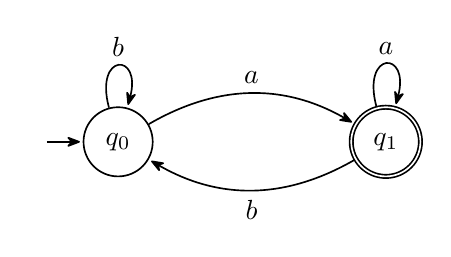
\begin{tikzpicture}[->,>={Stealth[round]},shorten >=1pt,auto,
                    node distance=3.4cm,semithick,initial text=]
  \node[state,initial]   (q0) {$q_0$};
  \node[state,accepting] (q1) [right of=q0] {$q_1$};
  \path (q0) edge[bend left] node {$a$} (q1)
        (q0) edge[loop above] node {$b$} (q0)
        (q1) edge[loop above] node {$a$} (q1)
        (q1) edge[bend left]  node {$b$} (q0);
\end{tikzpicture}
\caption{The derivative automaton of $r=(a+b)^{*}\cdot a$, with initial state
$q_0=[(a+b)^{*}\cdot a]$ and accepting state $q_1=[(a+b)^{*}\cdot a+\varepsilon]$.
Each edge is a canonical one-step derivative, $\delta(q,x)=[\mathcal{D}_x(q)]$.}
\label{fig:deriv-dfa}
\end{figure}

\medskip
\noindent\textbf{Example (with and without canonicalisation).}
This example shows exactly why canonicalisation matters.
Take $\Sigma=\{a\}$ and $r=a^{*}$.

With canonicalisation, the start state is $q_0=[a^{*}]=a^{*}$, and
$\mathcal{D}_a(a^{*})=\varepsilon\cdot a^{*}\sim a^{*}$, so
$\delta(q_0,a)=[a^{*}]=q_0$. The queue empties at once and the construction returns
the one-state automaton.

\begin{center}
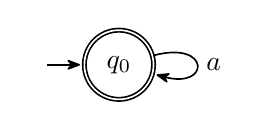
\begin{tikzpicture}[->,>={Stealth[round]},shorten >=1pt,auto,semithick,initial text=]
  \node[state,initial,accepting] (q0) {$q_0$};
  \path (q0) edge[loop right] node {$a$} (q0);
\end{tikzpicture}
\end{center}

Without canonicalisation, states are compared as raw syntax. Reading $a$ gives
$s_1=\varepsilon\cdot a^{*}$, then $s_2=\mathcal{D}_a(s_1)$, then $s_3$, each larger
than the last. Every $s_i$ denotes $a^{*}$ and every pair is similar, yet no two are
syntactically equal, so the construction never terminates. Canonicalisation collapses
this chain to the single representative $a^{*}$.

\begin{center}
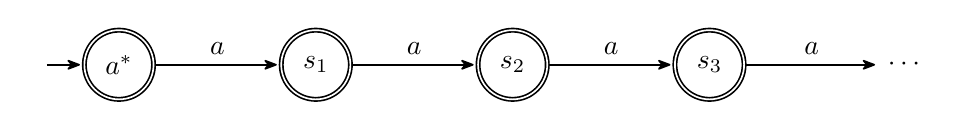
\begin{tikzpicture}[->,>={Stealth[round]},shorten >=1pt,auto,semithick,
                    initial text=,node distance=2.5cm]
  \node[state,initial,accepting] (q0) {$a^{*}$};
  \node[state,accepting] (s1) [right of=q0] {$s_1$};
  \node[state,accepting] (s2) [right of=s1] {$s_2$};
  \node[state,accepting] (s3) [right of=s2] {$s_3$};
  \node (dots) [right of=s3] {$\cdots$};
  \path (q0) edge node {$a$} (s1)
        (s1) edge node {$a$} (s2)
        (s2) edge node {$a$} (s3)
        (s3) edge node {$a$} (dots);
\end{tikzpicture}
\end{center}

\subsection{Fuzzy Proximity and Similarity Relations}\label{sec:fuzzy-relations}

The fuzzy setting compares symbols by degree rather than by equality. The first
ingredient is a way of combining degrees of similarity, namely a
T-norm~\cite{met05}.

\begin{definition}[T-norm]
A \emph{T-norm} is a binary operation $\otimes:[0,1]\times[0,1]\to[0,1]$ such that,
for all $x,y,z\in[0,1]$:
\begin{enumerate}
  \item \textbf{Commutativity:} $x\otimes y = y\otimes x$;
  \item \textbf{Associativity:} $(x\otimes y)\otimes z = x\otimes (y\otimes z)$;
  \item \textbf{Monotonicity:} if $x\le y$, then $x\otimes z \le y\otimes z$;
  \item \textbf{Neutral element:} $x\otimes 1 = x$.
\end{enumerate}
\end{definition}

\noindent We work with Gödel's T-norm.

\medskip
The development formalises a T-norm as a record \texttt{T\_norm} bundling
the axioms above, together with the requirement that the operation maps $[0,1]$ back
into $[0,1]$, and provides Gödel's minimum \texttt{smin} as the instance
\texttt{godel\_t\_norm}, whose record fields are proved by the corresponding lemmas
about \texttt{smin}.

\begin{lstlisting}[style=rocqstyle,caption={T-norms and Gödel's minimum (\texttt{SimilarityRelations.v}).},label={lst:tnorm}]
Definition simval := R.

Definition in01 (x : simval) : Prop := 0 <= x <= 1.

Record T_norm : Type := {
  tnorm : simval -> simval -> simval;
  tnorm_closed :
    forall x y, in01 x -> in01 y -> in01 (tnorm x y);
  tnorm_comm :
    forall x y, in01 x -> in01 y -> tnorm x y = tnorm y x;
  tnorm_assoc :
    forall x y z, in01 x -> in01 y -> in01 z ->
      tnorm (tnorm x y) z = tnorm x (tnorm y z);
  tnorm_mono_l :
    forall x y z, in01 x -> in01 y -> in01 z ->
      x <= y -> tnorm x z <= tnorm y z;
  tnorm_neutral_r :
    forall x, in01 x -> tnorm x 1 = x
}.

(* Godel's minimum T-norm *)
Definition smin (x y : simval) : simval :=
  if Rle_dec x y then x else y.

Definition godel_t_norm : T_norm :=
  {| tnorm := smin;
     tnorm_closed := smin_in010;
     tnorm_comm := fun x y _ _ => smin_comm0 x y;
     tnorm_assoc := fun x y z _ _ _ => smin_assoc0 x y z;
     tnorm_mono_l := fun x y z _ _ _ Hxy => @smin_mono_l0 x y z Hxy;
     tnorm_neutral_r := smin1r |}.
\end{lstlisting}

\begin{definition}[Fuzzy relation, cut, proximity, similarity]\mbox{}
\begin{enumerate}
\item A binary \emph{fuzzy relation} on a set $S$ is a mapping
$\mathcal{R}:S\times S\to[0,1]$. If $\mathcal{R}$ is a fuzzy relation on $S$ and
$\mu$ is a number $0<\mu\le 1$ (a \emph{cut value}), then the \emph{$\mu$-cut} of
$\mathcal{R}$, denoted $\mathcal{R}_\mu$, is the crisp relation
\[
  \mathcal{R}_\mu := \{(s_1,s_2)\mid \mathcal{R}(s_1,s_2)\ge\mu\}.
\]
\item A fuzzy relation $\mathcal{R}$ on $S$ is a \emph{proximity relation} if it is
reflexive and symmetric:
\begin{description}
  \item[Reflexivity:] $\mathcal{R}(s,s)=1$ for all $s\in S$;
  \item[Symmetry:] $\mathcal{R}(s_1,s_2)=\mathcal{R}(s_2,s_1)$ for all
        $s_1,s_2\in S$.
\end{description}
\item Let $\otimes$ be a left-continuous T-norm on $[0,1]$. A proximity relation is
a \emph{($T$-)similarity relation} iff it satisfies the reverse triangle inequality
with respect to $\otimes$:
\begin{description}
  \item[Reverse triangle inequality:]
        $\mathcal{R}(s_1,s_2)\ge \mathcal{R}(s_1,s)\otimes\mathcal{R}(s,s_2)$ for all
        $s_1,s_2,s\in S$.
\end{description}
\end{enumerate}
\end{definition}

With Gödel's minimum T-norm as $\otimes$, the symbol $\min$ is often written instead
of $\otimes$. These notions are those used in similarity-based approximate
reasoning~\cite{Sessa2002}. In Rocq the cut is \texttt{mu\_cut}, a proximity is the
record \texttt{is\_proximity}, and a similarity relation with respect to a given
T-norm \texttt{T} is the record \texttt{is\_T\_similarity T}, which records that
\texttt{T} is left-continuous and that the reverse triangle inequality holds with
respect to \texttt{tnorm T}.

\noindent\textbf{Example.} Take $\Sigma=\{a,b,c,d\}$ and let $\mathcal{R}$ assign
$\mathcal{R}(x,x)=1$ for every $x$, $\mathcal{R}(a,c)=\mathcal{R}(c,a)=0.9$,
$\mathcal{R}(b,d)=\mathcal{R}(d,b)=0.75$, and $0$ to every other distinct pair. This
$\mathcal{R}$ is a proximity relation, since it is reflexive and symmetric, and a
similarity relation under the minimum, since the only nontrivial chains pass through
a repeated symbol. Its cut depends on the threshold. At $\mu=0.8$ the cut
$\mathcal{R}_{0.8}$ relates $a$ with $c$ but leaves $b$ and $d$ apart, whereas at
$\mu=0.7$ the cut $\mathcal{R}_{0.7}$ relates both $a$ with $c$ and $b$ with $d$.

\begin{lstlisting}[style=rocqstyle,caption={Fuzzy relations, cut, proximity, and $T$-similarity (\texttt{SimilarityRelations.v}).},label={lst:fuzzyrel}]
Definition cut_value (mu : simval) : Prop := 0 < mu /\ mu <= 1.

Section FuzzyRelationLayer.
  Variable S : Type.

  (* Fuzzy relation *)
  Definition fuzzy_rel := S -> S -> simval.

  (* Fuzzy relation range *)
  Definition is_fuzzy_rel (R : fuzzy_rel) : Prop :=
    forall s1 s2, in01 (R s1 s2).

  (* mu-cut *)
  Definition mu_cut (mu : simval) (R : fuzzy_rel) : S -> S -> Prop :=
    fun s1 s2 => mu <= R s1 s2.

  (* Proximity relation *)
  Record is_proximity (R : fuzzy_rel) : Prop := {
    prox_range : is_fuzzy_rel R;
    prox_refl : forall s, R s s = 1;
    prox_sym  : forall s1 s2, R s1 s2 = R s2 s1
  }.

  (* T-similarity relation *)
  Record is_T_similarity (T : T_norm) (R : fuzzy_rel) : Prop := {
    tsim_left_continuous : left_continuous_on_01 (tnorm T);
    tsim_prox : is_proximity R;
    tsim_trans : forall s1 s2 s,
      tnorm T (R s1 s) (R s s2) <= R s1 s2
  }.
End FuzzyRelationLayer.
\end{lstlisting}

A base similarity relation between symbols,
$\mathcal{R}:\Sigma\times\Sigma\to[0,1]$, induces similarities between words and
between languages.

\begin{definition}[Similarity on words]\label{def:Rw}
Given a similarity relation $\mathcal{R}$ on $\Sigma$, define a proximity relation
on words $\mathcal{R}^{w}:\Sigma^{*}\times\Sigma^{*}\to[0,1]$ by
\[
\mathcal{R}^{w}(w_1,w_2)=
\begin{cases}
\bigotimes_{1\le i\le n}\mathcal{R}(a_i,b_i)
  & \text{if } w_1=a_1\cdots a_n \text{ and } w_2=b_1\cdots b_n;\\[0.4ex]
0 & \text{otherwise.}
\end{cases}
\]
\end{definition}

\noindent\textbf{Example.} With the base relation $\mathcal{R}$ of the previous
example and the minimum T-norm,
$\mathcal{R}^{w}(ab,cd)=\min(\mathcal{R}(a,c),\mathcal{R}(b,d))=\min(0.9,0.75)=0.75$,
while $\mathcal{R}^{w}(ab,cb)=\min(\mathcal{R}(a,c),\mathcal{R}(b,b))=\min(0.9,1)=0.9$.
The words $ab$ and $a$ have different lengths, so $\mathcal{R}^{w}(ab,a)=0$.

\begin{lstlisting}[style=rocqstyle,caption={Similarity on words (\texttt{SimilarityRelations.v}).},label={lst:Rw}]
Fixpoint Rw_T (T : T_norm) (w1 w2 : word) : simval :=
  match w1, w2 with
  | [::], [::] => 1
  | [::], _    => 0
  | _   , [::] => 0
  | a1 :: t1, a2 :: t2 =>
      tnorm T (R a1 a2) (Rw_T T t1 t2)
  end.
\end{lstlisting}

\begin{definition}[Similarity on languages]\label{def:RL}
For languages $L_1,L_2\subseteq\Sigma^{*}$ define a proximity relation
$\mathcal{R}^{L}:\mathcal{P}(\Sigma^{*})\times\mathcal{P}(\Sigma^{*})\to[0,1]$ by
\[
\mathcal{R}^{L}(L_1,L_2)=
\min\!\Bigl\{
\inf_{w_1\in L_1}\ \sup_{w_2\in L_2}\ \mathcal{R}^{w}(w_1,w_2)\,,\
\inf_{w_2\in L_2}\ \sup_{w_1\in L_1}\ \mathcal{R}^{w}(w_1,w_2)
\Bigr\}.
\]
\end{definition}

\noindent\textbf{Example.} Continuing with the same $\mathcal{R}$ and the minimum,
compare $L_1=\{ab\}$ and $L_2=\{cd,cb\}$. In the direction from $L_1$, the single
word $ab$ has $\sup\{\mathcal{R}^{w}(ab,cd),\mathcal{R}^{w}(ab,cb)\}=\max(0.75,0.9)=0.9$,
so the infimum over $L_1$ is $0.9$. In the direction from $L_2$, the word $cd$ gives
$\sup\{\mathcal{R}^{w}(ab,cd)\}=0.75$ and $cb$ gives
$\sup\{\mathcal{R}^{w}(ab,cb)\}=0.9$, so the infimum over $L_2$ is
$\min(0.75,0.9)=0.75$. The language similarity is the minimum of the two directions,
$\mathcal{R}^{L}(L_1,L_2)=\min(0.9,0.75)=0.75$.

\begin{lstlisting}[style=rocqstyle,caption={Similarity on languages (\texttt{SimilarityRelations.v}).},label={lst:RL}]
Definition RL_T (L1 L2 : language) : simval :=
  smin
    (@InfL L1
      (fun w1 =>
         @SupL L2 (fun w2 => Rw_T T w1 w2)
           (Rw_T_upper_bounded_right w1 L2))
      (outer_T_lower_bounded_left L1 L2))
    (@InfL L2
      (fun w2 =>
         @SupL L1 (fun w1 => Rw_T T w1 w2)
           (Rw_T_upper_bounded_left w2 L1))
      (outer_T_lower_bounded_right L1 L2)).
\end{lstlisting}

Viewing words as regular expressions, Definition~\ref{def:Rw} extends to
regular expressions when Gödel's T-norm is used.

\begin{definition}[Similarity on regular expressions, Gödel's T-norm]\label{def:Rexp-godel}
Given a similarity relation $\mathcal{R}$ on the alphabet, define a proximity on
regular expressions $\mathcal{G}^{E}:E^{\Sigma}\times E^{\Sigma}\to[0,1]$ by
\[
\mathcal{G}^{E}(r_1,r_2)=
\begin{cases}
\bigotimes_{1\le i\le n}\mathcal{R}(a_i,b_i)
  & \text{if } r_1=r[a_1,\ldots,a_n] \text{ and } r_2=r[b_1,\ldots,b_n];\\[0.4ex]
0 & \text{otherwise.}
\end{cases}
\]
\end{definition}

In Rocq this is the recursive function \texttt{GE}. It recurses on the shape of the
two expressions, returns the base similarity \texttt{R} on letters, the minimum on
matching binary shapes, and $0$ when the shapes differ.

\begin{lstlisting}[style=rocqstyle,caption={Gödel similarity on regular expressions (\texttt{SimilarityRelations.v}).},label={lst:GE}]
Fixpoint GE (r s : regex) : simval :=
  match s with
  | RS.Empty =>
      match r with
      | RS.Empty => 1
      | _ => 0
      end
  | RS.Eps =>
      match r with
      | RS.Eps => 1
      | _ => 0
      end
  | RS.Char a =>
      match r with
      | RS.Char b => R b a
      | _ => 0
      end
  | RS.Star s1 =>
      match r with
      | RS.Star r1 => GE r1 s1
      | _ => 0
      end
  | RS.Seq s1 s2 =>
      match r with
      | RS.Seq r1 r2 => smin (GE r1 s1) (GE r2 s2)
      | _ => 0
      end
  | RS.Alt s1 s2 =>
      match r with
      | RS.Alt r1 r2 => smin (GE r1 s1) (GE r2 s2)
      | _ => 0
      end
  end.
\end{lstlisting}

For arbitrary T-norms Definition~\ref{def:Rexp-godel} is too generous over regular
expressions. If $\mathcal{R}(a,b)\lneq 1$ then
$\mathcal{R}^{L}(\mathcal{L}(a^{*}),\mathcal{L}(b^{*}))=\mathcal{R}(a,b)$ only when
$\mathcal{R}(a,b)$ is idempotent; but a T-norm all of whose values are idempotent is
necessarily Gödel's minimum. There are nonetheless many non-idempotent T-norms one
wishes to consider, for example
\[
T(x,y)=
\begin{cases}
p+\dfrac{(x-p)(y-p)}{1-p} & x,y\ge p;\\[1.0ex]
\min(x,y) & \text{otherwise,}
\end{cases}
\]
where $p\in[0,1]$. Definition~\ref{def:Rexp-godel} ergo has to be
conservatively extended.

\begin{definition}[Similarity on regular expressions, general T-norm]\label{def:Re}
Let $r,s$ be restricted regular expressions over $\Sigma$ and $\mathcal{R}$ a
similarity on $\Sigma$. Define inductively the proximity relation
\[
\mathcal{R}^{e}(r,s)=
\begin{cases}
1 & \text{if } r=s;\\[0.3ex]
\mathcal{R}(a,b) & \text{if } r=a \text{ and } s=b;\\[0.3ex]
\min\{\mathcal{R}^{e}(r_1,s_1),\mathcal{R}^{e}(r_2,s_2)\}
  & \text{if } r=r_1+r_2 \text{ and } s=s_1+s_2;\\[0.3ex]
\mathcal{R}^{e}(r_1,s_1)\otimes\mathcal{R}^{e}(r_2,s_2)
  & \text{if } r=r_1\cdot r_2 \text{ and } s=s_1\cdot s_2;\\[0.3ex]
\inf_n\bigl(\textstyle\bigotimes^{n}\mathcal{R}^{e}(r_1,s_1)\bigr)
  & \text{if } r=r_1^{*} \text{ and } s=s_1^{*};\\[0.3ex]
0 & \text{otherwise.}
\end{cases}
\]
\end{definition}

The clause for $(\ )^{*}$ is strict for a general T-norm, but no definition
for a general T-norm seems reasonable unless it is replaced by a finite union. In
Rocq this is the recursive function \texttt{RE\_T}, parameterised by the T-norm
\texttt{T}. The union and concatenation clauses both combine the subexpression
values with \texttt{tnorm T}, and the star clause uses \texttt{tnorm\_power\_inf T},
the infimum of the T-norm powers $\inf_n(\bigotimes^{n}x)$. Under Gödel's minimum,
which is idempotent, \texttt{tnorm\_power\_inf} collapses to the identity and
\texttt{RE\_T} reduces to \texttt{GE}.

\begin{lstlisting}[style=rocqstyle,caption={Syntactic similarity on expressions, general T-norm (\texttt{SimilarityRelations.v}).},label={lst:rr}]
Fixpoint RE_T (r s : regex) {struct s} : simval :=
  match s with
  | RS.Empty =>
      match r with
      | RS.Empty => 1
      | _ => 0
      end
  | RS.Eps =>
      match r with
      | RS.Eps => 1
      | _ => 0
      end
  | RS.Char b =>
      match r with
      | RS.Char a => R a b
      | _ => 0
      end
  | RS.Alt s1 s2 =>
      match r with
      | RS.Alt r1 r2 => tnorm T (RE_T r1 s1) (RE_T r2 s2)
      | _ => 0
      end
  | RS.Seq s1 s2 =>
      match r with
      | RS.Seq r1 r2 => tnorm T (RE_T r1 s1) (RE_T r2 s2)
      | _ => 0
      end
  | RS.Star s1 =>
      match r with
      | RS.Star r1 => tnorm_power_inf T (RE_T r1 s1)
      | _ => 0
      end
  end.
\end{lstlisting}

\noindent\textbf{Example.} With the same base relation and the minimum, comparing
expressions of matching shape gives
$\mathcal{R}^{e}(a\cdot b,\,c\cdot d)=\min(\mathcal{R}(a,c),\mathcal{R}(b,d))=\min(0.9,0.75)=0.75$
and $\mathcal{R}^{e}(a\cdot b,\,c\cdot b)=\min(0.9,1)=0.9$, while a star gives
$\mathcal{R}^{e}(a^{*},c^{*})=\mathcal{R}(a,c)=0.9$ because the minimum is
idempotent. When the shapes differ the value is $0$, for instance
$\mathcal{R}^{e}(a\cdot b,\,c+d)=0$ since one expression is a concatenation and the
other a union.

\medskip
The three constructions are all similarity relations.

\begin{lemma}\label{lem:sim-relations}\mbox{}
\begin{enumerate}
\item $\mathcal{R}^{e}$ is a similarity relation on $E^{\Sigma}$, and therefore on
restricted regular expressions;
\item $\mathcal{R}^{w}$ is a similarity relation on $\Sigma^{*}$;
\item $\mathcal{R}^{L}$ is a similarity relation on languages.
\end{enumerate}
\end{lemma}

\begin{proof}
All three are formalised, and bundled together in the lemma
\texttt{general\_\allowbreak similarity\_\allowbreak relations} of
Listing~\ref{lst:simproofs}. Fix any
T-norm \texttt{T} that is left-continuous and with respect to which the base
relation \texttt{R} is transitive. Then $\mathcal{R}^{e}$, $\mathcal{R}^{w}$ and
$\mathcal{R}^{L}$ are all $T$-similarity relations. Each is proved by induction.
For words the induction is on the length, and transitivity follows because the
head and the tail can be combined through the monotonicity of the T-norm. For
expressions the induction is on the shape that the two share. For languages the
result is read off from the word case, using that a language similarity is built
from suprema and infima of word similarities.
\end{proof}

\begin{lstlisting}[style=rocqstyle,escapeinside={(@}{@)},caption={The three similarity relations, formalised (\texttt{SimilarityRelations.v}).},label={lst:simproofs}]
(* Similarity relations on restricted regular expressions, words, and languages. *)
Lemma general_similarity_relations :
  forall T,
    left_continuous_on_01 (tnorm T) ->
    (forall a b c, tnorm T (R a b) (R b c) <= R a c) ->
    @is_T_similarity restricted_regex_type T (RE_T_restricted T) /\
    @is_T_similarity word T (Rw_T T) /\
    @is_T_similarity language T (RL_T T).
(* Proof in SimilarityRelations.v of the repository (@\cite{OurRocqRepo}@). *)
\end{lstlisting}

\begin{remark}\label{rem:syntax-sensitive}\mbox{}
\begin{enumerate}
\item Definition~\ref{def:Re} is syntax-sensitive. Two regular expressions may
denote the same language while having low, or even zero, $\mathcal{R}^{e}$-similarity.
For example, depending on the base relation, $\mathcal{R}^{e}(a+b,b+a)=0$ even though
$\mathcal{L}(a+b)=\mathcal{L}(b+a)$.
\item For $r_1,r_2\in R^{\Sigma}$ and words $w_1\in\mathcal{L}(r_1)$,
$w_2\in\mathcal{L}(r_2)$ of the same length, $\mathcal{R}^{e}(r_1,r_2)$ and
$\mathcal{R}^{w}(w_1,w_2)$ are in general incomparable: $\mathcal{R}^{w}(a,a)=1$ but
$\mathcal{R}^{e}(a,a+a)=0$, while $\mathcal{R}^{w}(a,b)=0$ but
$\mathcal{R}^{e}(a+b,a+b)=1$.
\item One may build finite equational properties into the definition, for instance
setting $\mathcal{R}^{e}(r_1,s)=\mathcal{R}^{e}(r_2,s)$ whenever
$\mathsf{nf}(r_1)=\mathsf{nf}(r_2)$, but no exhaustive finitary definition is
possible, and this is not pursued here.
\item The bound $\mathcal{R}^{e}(r_1,r_2)\le\mathcal{R}^{L}(\mathcal{L}(r_1),\mathcal{L}(r_2))$
fails once $\&$ and $\neg$ are allowed. If
$\mathcal{R}(a,b)\gneq 0$ but $a\neq b$, then $\mathcal{L}(a\,\&\,b)=\emptyset$, so
$\mathcal{R}^{L}(\mathcal{L}(a\,\&\,a),\mathcal{L}(a\,\&\,b))=0$, whereas a
shape-based value $\mathcal{R}^{e}(a\,\&\,a,a\,\&\,b)=\mathcal{R}(a,b)>0$. This is
why the fuzzy theory is confined to the restricted fragment $R^{\Sigma}$.
\end{enumerate}
\end{remark}

\begin{lemma}[Finite syntactic similarity]\label{lem:finite-syntactic}
If $\Sigma$ is finite, then for every restricted regular expression $r$ the set
$\{\,s \mid \mathcal{R}^{e}(s,r)\neq 0\,\}$ is finite.
\end{lemma}

\begin{proof}
This is formalised as the lemma \texttt{finite\_syntactic\_similarity} of
Listing~\ref{lst:finite}. The development builds a finite list
\texttt{syntactic\_similarity\_candidates alphabet r}, which enumerates all
expressions sharing the outermost shape of $r$ with letters drawn from the
alphabet, and proves, by induction on the derivation that $r$ is restricted, that
every $s$ with $\mathcal{R}^{e}(s,r)\neq 0$ (that is, $\texttt{RE\_T}\ T\ s\ r\neq0$)
belongs to that list. The base cases use that for letters only the finitely many
$b$ with $\mathcal{R}(b,a)\neq 0$ qualify, and the inductive cases use that the
T-norm is non-zero only when both arguments are. Since the candidate list is finite,
so is $\{s\mid\mathcal{R}^{e}(s,r)\neq 0\}$.
\end{proof}

\begin{lstlisting}[style=rocqstyle,escapeinside={(@}{@)},caption={Finiteness of syntactic similarity, formalised (\texttt{SimilarityRelations.v}).},label={lst:finite}]
Fixpoint syntactic_similarity_candidates
  (alphabet : list A) (r : regex) : list regex :=
  match r with
  | RS.Empty => (RS.Empty :: nil)%list
  | RS.Eps => (RS.Eps :: nil)%list
  | RS.Char _ => List.map RS.Char alphabet
  | RS.Alt r1 r2 =>
      List.flat_map
        (fun s1 =>
           List.map (fun s2 => RS.Alt s1 s2)
             (syntactic_similarity_candidates alphabet r2))
        (syntactic_similarity_candidates alphabet r1)
  | RS.Seq r1 r2 =>
      List.flat_map
        (fun s1 =>
           List.map (fun s2 => RS.Seq s1 s2)
             (syntactic_similarity_candidates alphabet r2))
        (syntactic_similarity_candidates alphabet r1)
  | RS.Star r1 =>
      List.map RS.Star
        (syntactic_similarity_candidates alphabet r1)
  end.

(* Finite Syntactic Similarity *)
Lemma finite_syntactic_similarity :
  forall T alphabet r,
    (forall a, List.In a alphabet) ->
    RS.restricted_regex r ->
    forall s,
      RE_T T s r <> 0 ->
      List.In s (syntactic_similarity_candidates alphabet r).
(* Proof in SimilarityRelations.v of the repository (@\cite{OurRocqRepo}@). *)
\end{lstlisting}


\subsection{Fuzzy Derivatives and Fuzzy Automata}\label{sec:fuzzy-derivatives}

The derivative now carries over to the fuzzy setting. Comparing only the consumed
symbol with the first symbol of a word in the language would be too narrow. In a
similarity-based setting the remaining suffix should also be matched up to the same
cut, so the whole word is matched. Formalising the fuzzy derivative and the fuzzy
automaton in Rocq is ongoing research.

\begin{definition}[Fuzzy language derivative]\label{def:fuzzy-deriv-lang}
Let $\mathcal{L}\subseteq\Sigma^{*}$, $a\in\Sigma$ and $0<\mu\le1$. The
\emph{$\mu$-fuzzy derivative} of $\mathcal{L}$ with respect to $a$ is
\[
\partial_a^{\mu}(\mathcal{L})
= \{\,w\in\Sigma^{*} \mid \exists\, b\in\Sigma,\ \exists\, v\in\Sigma^{*}
   \text{ such that } \mathcal{R}(a,b)\otimes\mathcal{R}^{w}(w,v)\ge\mu
   \text{ and } bv\in\mathcal{L}\,\}.
\]
\end{definition}

\begin{definition}[Fuzzy expression derivative]\label{def:fuzzy-deriv-expr}
Let $r$ be a restricted regular expression over $\Sigma$, $a\in\Sigma$ and
$0<\mu\le1$. The \emph{fuzzy derivative} of $r$ with respect to $a$ and $\mu$ is
\[
\mathcal{D}_a^{\mu}(r)
= \sum_{\mathcal{R}(a,b)\otimes\mathcal{R}^{e}(s,r)\ge\mu} \mathcal{D}_b(s),
\]
where $\mathcal{D}_b(s)$ is the ordinary Brzozowski derivative of
Section~\ref{sec:crisp-derivatives}.
\end{definition}

\noindent\textbf{Example.} With $\mathcal{R}(a,c)=0.9$, the other values as in the
running example, $\mu=0.7$ and $r=a$, the symbols $\mu$-similar to $a$ are $a$ and
$c$, and the expressions $\mu$-similar to $a$ are likewise $a$ and $c$. The sum
therefore ranges over $b,s\in\{a,c\}$ and gives
\[
\mathcal{D}_a^{\mu}(a)
= \mathcal{D}_a(a)+\mathcal{D}_c(c)+\mathcal{D}_c(a)+\mathcal{D}_a(c)
= \varepsilon+\varepsilon+\emptyset+\emptyset,
\]
which canonicalises to $\varepsilon$.

\begin{definition}[Fuzzy derivative with respect to a word]\label{def:fuzzy-word-deriv}
For a word $u=av$ with $a\in\Sigma$ and $v\in\Sigma^{*}$, the fuzzy derivatives of a
language and of a restricted regular expression with respect to $u$ are
\[
\partial_u^{\mu}(\mathcal{L})
= \bigcup_{\mu'\otimes\mu''\ge\mu}\partial_v^{\mu'}\bigl(\partial_a^{\mu''}(\mathcal{L})\bigr),
\qquad
\mathcal{D}_u^{\mu}(r)
= \sum_{\mu'\otimes\mu''\ge\mu}\mathcal{D}_v^{\mu'}\bigl(\mathcal{D}_a^{\mu''}(r)\bigr),
\]
with $\mathcal{D}_\varepsilon^{\mu}(r)=r$.
\end{definition}

Both expression derivatives are syntactic. By
Lemma~\ref{lem:finite-syntactic} the summands in the sums are finite, so
$\mathcal{D}_u^{\mu}(r)$ is a well-defined restricted regular expression.

From now on $\otimes$ is Gödel's minimum T-norm. Its idempotence makes
the cut relations equivalences, which is what reduces the fuzzy theory to the
crisp one.

\begin{proposition}[Cut equivalences]\label{prop:cut-equivalence}
Let $\mathcal{R}$ be a fuzzy similarity relation on $\Sigma$ and $0<\mu\le1$. Each of
the relations
\[
a\sim_\mu^{\Sigma} b \iff \mathcal{R}(a,b)\ge\mu, \qquad
r\sim_\mu^{e} s \iff \mathcal{R}^{e}(r,s)\ge\mu,
\]
\[
w_1\sim_\mu^{\Sigma^{*}} w_2 \iff \mathcal{R}^{w}(w_1,w_2)\ge\mu, \qquad
L_1\sim_\mu^{\mathcal{P}(\Sigma^{*})} L_2 \iff \mathcal{R}^{L}(L_1,L_2)\ge\mu,
\]
on symbols, restricted expressions, words and languages respectively, is an
equivalence relation. Moreover $a_1\cdots a_n\sim_\mu^{\Sigma^{*}} b_1\cdots b_m$ if
and only if $n=m$ and $a_i\sim_\mu^{\Sigma} b_i$ for every $i$.
\end{proposition}

Under the minimum, the condition $\mathcal{R}(a,b)\otimes\mathcal{R}^{w}(w,v)\ge\mu$
splits into $\mathcal{R}(a,b)\ge\mu$ and $\mathcal{R}^{w}(w,v)\ge\mu$, that is
$(a,b)\in\mathcal{R}_\mu$ and $w\sim_\mu^{\Sigma^{*}} v$, so the fuzzy language
derivative reads
\[
\partial_a^{\mu}(\mathcal{L})
= \{\,w\mid \exists\, b,v:\ (a,b)\in\mathcal{R}_\mu,\ w\sim_\mu^{\Sigma^{*}} v,\ bv\in\mathcal{L}\,\}.
\]

\begin{definition}[Cut neighbourhood]\label{def:cut-neighborhood}
For $a\in\Sigma$ and $0<\mu\le1$, the \emph{cut neighbourhood} of $a$ is
$\mathcal{S}_a^{\mu}=\{\,b\in\Sigma\mid (a,b)\in\mathcal{R}_\mu\,\}$, that is, the
$\mu$-equivalence class of $a$.
\end{definition}

\begin{definition}[Quotient alphabet and language]\label{def:quotient}
Let $\Sigma^{\mu}:=\Sigma/{\sim_\mu^{\Sigma}}$ and let $q_\mu:\Sigma\to\Sigma^{\mu}$,
$q_\mu(a)=[a]_\mu$, be the quotient map, extended to words letterwise by
$q_\mu^{*}(a_1\cdots a_n)=[a_1]_\mu\cdots[a_n]_\mu$. For a language
$\mathcal{L}\subseteq\Sigma^{*}$, its \emph{quotient image} is
$\mathcal{L}^{\mu}:=q_\mu^{*}(\mathcal{L})=\{q_\mu^{*}(w)\mid w\in\mathcal{L}\}
\subseteq(\Sigma^{\mu})^{*}$.
\end{definition}

Once letters are identified up to
$\mu$-similarity, the fuzzy derivative becomes an ordinary derivative over the
quotient alphabet.

\begin{theorem}[Quotient form of the fuzzy derivative]\label{the:quotient-fuzzy-derivative}
For every language $\mathcal{L}\subseteq\Sigma^{*}$ and every $a\in\Sigma$,
\[
\partial_a^{\mu}(\mathcal{L})
= \{\,w\in\Sigma^{*}\mid q_\mu^{*}(w)\in\partial_{[a]_\mu}(\mathcal{L}^{\mu})\,\},
\qquad\text{ergo}\qquad
q_\mu^{*}\bigl(\partial_a^{\mu}(\mathcal{L})\bigr)=\partial_{[a]_\mu}\bigl(\mathcal{L}^{\mu}\bigr).
\]
\end{theorem}

\begin{proof}
The two inclusions are proved as follows. Let $w\in\partial_a^{\mu}(\mathcal{L})$. There are
$b\in\Sigma$ and $v\in\Sigma^{*}$ with $\mathcal{R}(a,b)\ge\mu$,
$w\sim_\mu^{\Sigma^{*}} v$ and $bv\in\mathcal{L}$. Then $[b]_\mu=[a]_\mu$ and
$q_\mu^{*}(w)=q_\mu^{*}(v)$, so
\[
[a]_\mu\, q_\mu^{*}(w)=[b]_\mu\, q_\mu^{*}(v)=q_\mu^{*}(bv)\in\mathcal{L}^{\mu},
\]
whence $q_\mu^{*}(w)\in\partial_{[a]_\mu}(\mathcal{L}^{\mu})$. Conversely, suppose
$q_\mu^{*}(w)\in\partial_{[a]_\mu}(\mathcal{L}^{\mu})$. Then
$[a]_\mu\, q_\mu^{*}(w)\in\mathcal{L}^{\mu}$, so there is a word $bv\in\mathcal{L}$
with $q_\mu^{*}(bv)=[a]_\mu\, q_\mu^{*}(w)$. Comparing first letters gives
$[b]_\mu=[a]_\mu$, i.e.\ $\mathcal{R}(a,b)\ge\mu$, and comparing the remainders gives
$q_\mu^{*}(v)=q_\mu^{*}(w)$, i.e.\ $w\sim_\mu^{\Sigma^{*}} v$; thus
$w\in\partial_a^{\mu}(\mathcal{L})$. The displayed consequence follows because
$\partial_{[a]_\mu}(\mathcal{L}^{\mu})$ consists only of quotient words, and each
such word has at least one representative in $\Sigma^{*}$.
\end{proof}

\noindent\textbf{Example.}
Let $\Sigma=\{a,b,c,d\}$ and let $\mathcal{R}$ be the similarity relation with
$\mathcal{R}(x,x)=1$ for every $x$, $\mathcal{R}(a,c)=\mathcal{R}(c,a)=0.9$,
$\mathcal{R}(b,d)=\mathcal{R}(d,b)=0.75$, and $\mathcal{R}(x,y)=0$ for all other
distinct $x,y$. Take the cut $\mu=0.7$. The $\mu$-cut is
\[
\mathcal{R}_\mu=\{(a,a),(b,b),(c,c),(d,d),(a,c),(c,a),(b,d),(d,b)\},
\]
so its classes are $[a]_\mu=\{a,c\}$ and $[b]_\mu=\{b,d\}$, and the quotient alphabet
is $\Sigma^{\mu}=\{[a]_\mu,[b]_\mu\}$.

Consider $\mathcal{L}=\{ab,\,cd,\,cb\}$. To compute $\partial_a^{\mu}(\mathcal{L})$,
collect the words of $\mathcal{L}$ whose first letter is $\mu$-similar to $a$,
that is, lies in $\{a,c\}$, and keep their suffixes up to $\mu$-similarity. All
three words $ab,cd,cb$ begin with a letter in $\{a,c\}$, leaving the suffixes
$b,d,b$, each of which is $\mu$-similar exactly to the words in $\{b,d\}$. Ergo
\[
\partial_a^{\mu}(\mathcal{L})=\{b,d\}=\partial_c^{\mu}(\mathcal{L}),
\]
the two being equal because $a\sim_\mu^{\Sigma} c$. No word of $\mathcal{L}$ begins
with a letter in the class $\{b,d\}$, so
$\partial_b^{\mu}(\mathcal{L})=\partial_d^{\mu}(\mathcal{L})=\emptyset$.

The quotient construction gives the same answer directly. Applying $q_\mu^{*}$
letterwise, $q_\mu^{*}(ab)=q_\mu^{*}(cd)=q_\mu^{*}(cb)=[a]_\mu[b]_\mu$, so
$\mathcal{L}^{\mu}=\{[a]_\mu[b]_\mu\}$. Its ordinary derivative with respect to
$[a]_\mu$ is $\partial_{[a]_\mu}(\mathcal{L}^{\mu})=\{[b]_\mu\}$, and taking the
inverse image under $q_\mu^{*}$ recovers
$(q_\mu^{*})^{-1}(\{[b]_\mu\})=\{b,d\}=\partial_a^{\mu}(\mathcal{L})$, exactly as
Theorem~\ref{the:quotient-fuzzy-derivative} predicts.

\medskip
The quotient viewpoint immediately yields closure under derivation.

\begin{theorem}[Regularity of fuzzy derivatives]\label{the:fuzzy-regular}
For every $u\in\Sigma^{*}$ and every $0<\mu\le1$, if $\mathcal{L}$ is regular then
$\partial_u^{\mu}(\mathcal{L})$ is regular; and if $r$ is restricted then
$\mathcal{D}_u^{\mu}(r)$ is a restricted regular expression.
\end{theorem}

\begin{proof}
Fix $0<\mu\le1$ and let $\mathcal{L}$ be regular. For a single symbol $a$,
Theorem~\ref{the:quotient-fuzzy-derivative} gives
$\partial_a^{\mu}(\mathcal{L})=(q_\mu^{*})^{-1}\bigl(\partial_{[a]_\mu}(\mathcal{L}^{\mu})\bigr)$.
Since $q_\mu^{*}$ is a homomorphism and $\mathcal{L}$ is regular, the quotient image
$\mathcal{L}^{\mu}$ is regular over the finite alphabet $\Sigma^{\mu}$; classical
derivatives preserve regularity (Theorem~\ref{the:language-derivative-regular}), so
$\partial_{[a]_\mu}(\mathcal{L}^{\mu})$ is regular; and the inverse homomorphic image
of a regular language is regular. Thus $\partial_a^{\mu}(\mathcal{L})$ is regular.
For a word $u=a_1\cdots a_n$ the same argument applies at each step of
$\partial_u^{\mu}(\mathcal{L})=\partial_{a_n}^{\mu}(\cdots\partial_{a_1}^{\mu}(\mathcal{L})\cdots)$,
so $\partial_u^{\mu}(\mathcal{L})$ is regular. The expression statement is immediate
from Definitions~\ref{def:fuzzy-deriv-expr} and~\ref{def:fuzzy-word-deriv}. Ordinary
Brzozowski derivatives are restricted regular expressions, and a finite sum of
restricted regular expressions is restricted.
\end{proof}

To relate the syntactic and semantic sides, an expression is interpreted up to
$\mu$-similarity.

\begin{definition}[Fuzzy semantic interpretation]\label{def:fuzzy-sem}
For a restricted regular expression $r$ and $0<\mu\le1$, the \emph{fuzzy semantic
interpretation} of $r$ is the language
\[
\mathcal{L}^{\mu}(r)=\{\,w\in\Sigma^{*}\mid w\sim_\mu^{\Sigma^{*}} v
   \text{ for some } v\in\mathcal{L}(r)\,\}.
\]
\end{definition}

\noindent\textbf{Example.} With the running data and $r=a\cdot b$, the language is
$\mathcal{L}(r)=\{ab\}$, and the words $\mu$-similar to $ab$ are exactly those $xy$
with $x\in\{a,c\}$ and $y\in\{b,d\}$, so
$\mathcal{L}^{\mu}(a\cdot b)=\{ab,ad,cb,cd\}$.

\begin{theorem}[Semantic--syntactic correspondence]\label{the:fuzzy-correspondence}
Let $r$ be a restricted regular expression over $\Sigma$, $u\in\Sigma^{*}$ and
$0<\mu\le1$. Then
$\mathcal{L}^{\mu}\bigl(\mathcal{D}_u^{\mu}(r)\bigr)=\partial_u^{\mu}\bigl(\mathcal{L}(r)\bigr)$.
\end{theorem}

\begin{proof}
First treat a single symbol $a$. By Definition~\ref{def:fuzzy-deriv-expr} and the
distributivity of the semantics over $+$,
\[
\mathcal{L}\bigl(\mathcal{D}_a^{\mu}(r)\bigr)
= \bigcup_{a\sim_\mu^{\Sigma} b,\ s\sim_\mu^{e} r}\mathcal{L}\bigl(\mathcal{D}_b(s)\bigr)
= \bigcup_{a\sim_\mu^{\Sigma} b,\ s\sim_\mu^{e} r}\partial_b\bigl(\mathcal{L}(s)\bigr),
\]
where the second equality is the crisp semantic--syntactic correspondence
(Theorem~\ref{the:two-derivative-mapping}). By Definition~\ref{def:Re} the relation
$s\sim_\mu^{e} r$ holds exactly when $s$ has the same shape as $r$ with each letter
replaced by a $\mu$-similar one, so as $b$ ranges over the class of $a$ and $s$ over
the class of $r$, the words $bv$ with $v\in\mathcal{L}(s)$ range exactly over the
words that are $\mu$-similar, letter by letter, to words of $\mathcal{L}(r)$ and
begin with a letter $\mu$-similar to $a$. Closing the displayed union under
$\mu$-similarity of the suffix ergo yields precisely the set described in
Definition~\ref{def:fuzzy-deriv-lang}, that is
$\mathcal{L}^{\mu}\bigl(\mathcal{D}_a^{\mu}(r)\bigr)=\partial_a^{\mu}\bigl(\mathcal{L}(r)\bigr)$.
For a word $u=av$ the argument is by induction on $|u|$. Using
Definitions~\ref{def:fuzzy-word-deriv} and the single-symbol case,
\[
\mathcal{L}^{\mu}\bigl(\mathcal{D}_u^{\mu}(r)\bigr)
= \partial_v^{\mu}\bigl(\partial_a^{\mu}(\mathcal{L}(r))\bigr)
= \partial_u^{\mu}\bigl(\mathcal{L}(r)\bigr),
\]
which completes the proof.
\end{proof}

A deterministic automaton for the fuzzy language can now be built exactly as in the
crisp case, taking canonical fuzzy derivatives as states. The first step is to see
that there are only finitely many of them.

\begin{theorem}[Finiteness of fuzzy language derivatives]\label{the:fuzzy-finite}
Let $\Sigma$ be finite and $0<\mu\le1$. If $\mathcal{L}\subseteq\Sigma^{*}$ is
regular, then the set $\bigl\{\,\partial_u^{\mu}(\mathcal{L})\mid u\in\Sigma^{*}\,\bigr\}$
is finite.
\end{theorem}

\begin{proof}
Since $q_\mu^{*}$ is a homomorphism, the quotient image $\mathcal{L}^{\mu}$ is a
regular language over the finite alphabet $\Sigma^{\mu}$. By
Theorem~\ref{the:derivative-set-is-finite} the set
$D^{\mu}=\{\,\partial_x(\mathcal{L}^{\mu})\mid x\in(\Sigma^{\mu})^{*}\,\}$ is finite.
By repeated application of Theorem~\ref{the:quotient-fuzzy-derivative}, every fuzzy
derivative has the form
$\partial_u^{\mu}(\mathcal{L})=(q_\mu^{*})^{-1}\bigl(\partial_{q_\mu^{*}(u)}(\mathcal{L}^{\mu})\bigr)$,
the inverse image of an element of the finite set $D^{\mu}$. Ergo
$\{\,\partial_u^{\mu}(\mathcal{L})\mid u\in\Sigma^{*}\,\}$ is finite.
\end{proof}

\begin{theorem}[Finiteness of fuzzy expression derivatives]\label{the:fuzzy-finite-expr}
Let $\Sigma$ be finite and $0<\mu\le1$. For a restricted regular expression $R$, the
set $\bigl\{\,\mathcal{L}^{\mu}(\mathcal{D}_w^{\mu}(R))\mid w\in\Sigma^{*}\,\bigr\}$
is finite.
\end{theorem}

\begin{proof}
By the semantic--syntactic correspondence (Theorem~\ref{the:fuzzy-correspondence}),
$\mathcal{L}^{\mu}(\mathcal{D}_w^{\mu}(R))=\partial_w^{\mu}(\mathcal{L}(R))$ for every
$w\in\Sigma^{*}$, so
\[
\bigl\{\,\mathcal{L}^{\mu}(\mathcal{D}_w^{\mu}(R))\mid w\in\Sigma^{*}\,\bigr\}
= \bigl\{\,\partial_w^{\mu}(\mathcal{L}(R))\mid w\in\Sigma^{*}\,\bigr\},
\]
and the right-hand set is finite by Theorem~\ref{the:fuzzy-finite}.
\end{proof}

Finiteness guarantees that the construction of Section~\ref{sec:dfa}, run with fuzzy
derivatives, terminates. The automaton recognises the words that lie
within tolerance $\mu$ of the language of $r$.

\begin{theorem}[Fuzzy DFA correctness]\label{the:fuzzy-dfa}
Let $r$ be a restricted regular expression over $\Sigma$, let $0<\mu\le1$, and let
$M^{\mu}=\langle Q^{\mu},\Sigma,\delta^{\mu},q_0^{\mu},F^{\mu}\rangle$ be the DFA
constructed from $r$ with fuzzy derivatives at cut $\mu$, that is, with
$q_0^{\mu}=[r]$, $\delta^{\mu}(q,a)=[\mathcal{D}_a^{\mu}(q)]$, and
$F^{\mu}=\{q\mid \nu(q)=\varepsilon\}$. Writing
\[
\mathcal{L}_\Sigma^{\mu}(r)=(q_\mu^{*})^{-1}\bigl(q_\mu^{*}(\mathcal{L}(r))\bigr)
\]
for the words that are $\mu$-similar to some word of $r$, the automaton satisfies
\[
\mathcal{L}(M^{\mu})=\mathcal{L}_\Sigma^{\mu}(r).
\]
\end{theorem}

\begin{proof}
Let $\delta^{\mu *}$ extend $\delta^{\mu}$ to words by
$\delta^{\mu *}(q,\varepsilon)=q$ and
$\delta^{\mu *}(q,wa)=\delta^{\mu}(\delta^{\mu *}(q,w),a)$. Induction on $w$
shows $\delta^{\mu *}(q_0^{\mu},w)=[\mathcal{D}_w^{\mu}(r)]$. For $w=\varepsilon$ this
is $q_0^{\mu}=[r]=[\mathcal{D}_\varepsilon^{\mu}(r)]$. For $w=ua$, the induction
hypothesis and the definition of $\delta^{\mu}$ give
\[
\delta^{\mu *}(q_0^{\mu},ua)
= \delta^{\mu}\bigl([\mathcal{D}_u^{\mu}(r)],a\bigr)
= [\mathcal{D}_a^{\mu}(\mathcal{D}_u^{\mu}(r))]
= [\mathcal{D}_{ua}^{\mu}(r)].
\]
Therefore, for any $w\in\Sigma^{*}$,
\[
\begin{aligned}
w \text{ accepted by } M^{\mu}
&\iff \delta^{\mu *}(q_0^{\mu},w)\in F^{\mu}
 \iff \nu(\mathcal{D}_w^{\mu}(r))=\varepsilon
 \iff \varepsilon\in\mathcal{L}(\mathcal{D}_w^{\mu}(r)) \\
&\iff \varepsilon\in\mathcal{L}^{\mu}(\mathcal{D}_w^{\mu}(r))
 \iff \varepsilon\in\partial_w^{\mu}(\mathcal{L}(r))
 \iff w\in\mathcal{L}_\Sigma^{\mu}(r),
\end{aligned}
\]
where the fourth step uses that the only word $\mu$-similar to $\varepsilon$ is
$\varepsilon$ itself, the fifth is Theorem~\ref{the:fuzzy-correspondence}, and the
last is the definition of $\mathcal{L}_\Sigma^{\mu}(r)$ together with the quotient
form of the fuzzy derivative. Ergo $\mathcal{L}(M^{\mu})=\mathcal{L}_\Sigma^{\mu}(r)$.
\end{proof}

\section{Conclusion}\label{sec:conclusion}

The question behind this thesis was whether the derivative-based theory of regular
languages still works once exact symbol matching is dropped and symbols are allowed
to match by similarity instead, and whether the core of that theory can be checked
by a machine rather than trusted on paper. The work in the preceding sections
answers yes to both.

On the crisp side the thesis gives a self-contained account of derivatives of
regular languages and of regular expressions. The result everything else rests on is
Theorem~\ref{the:two-derivative-mapping}, which says that the syntactic derivative
of an expression and the semantic derivative of its language describe the same
thing once an expression is read as the language it denotes. From there it is a
short step to the fact that derivatives stay regular and that an expression has only
finitely many derivative languages (Theorem~\ref{the:derivative-set-is-finite}).
That finiteness is exactly what makes the derivative automaton possible: taking
canonical derivatives as states and differentiation as the transition yields a
deterministic automaton that recognises the right language
(Theorem~\ref{the:dfa-correctness}) and that a terminating algorithm actually
builds.

The fuzzy layer is where the thesis makes its own contribution. Once equality of
symbols is replaced by a fuzzy similarity relation together with a cut value $\mu$,
fuzzy derivatives of both languages and restricted regular expressions arise
(Definitions~\ref{def:fuzzy-deriv-lang} and~\ref{def:fuzzy-deriv-expr}). The idea
that makes the whole layer tractable is small but decisive: under the minimum
T-norm, cut-similarity turns out to be an equivalence relation
(Proposition~\ref{prop:cut-equivalence}). Once that is in hand, a fuzzy derivative
over $\Sigma$ is just an ordinary derivative over the quotient alphabet
$\Sigma^{\mu}$ obtained by collapsing $\mu$-similar symbols into a single class
(Theorem~\ref{the:quotient-fuzzy-derivative}). This quotient picture is what lets
the crisp theory carry over almost without extra effort, so regularity
(Theorem~\ref{the:fuzzy-regular}), the correspondence between syntax and semantics
(Theorem~\ref{the:fuzzy-correspondence}), finiteness
(Theorem~\ref{the:fuzzy-finite}) and fuzzy DFA correctness
(Theorem~\ref{the:fuzzy-dfa}) all follow. In plain terms, the fuzzy automaton
accepts precisely the words that come within tolerance $\mu$ of some word in the
original language.

This quotient construction is really the point of the thesis. It does more than
confirm that the fuzzy theorems happen to hold; it explains why fuzzification by
cut-similarity behaves so well in the first place, and it makes the fuzzy derivative
something computable, since the computation collapses to ordinary derivatives
over a finite quotient alphabet. The verification side carries its own weight.
Mechanising the crisp theory in Rocq turns the central claims into statements a
proof assistant has checked, covering the syntax and semantics, nullability,
canonicalisation and its correctness, the derivative correspondence and DFA
correctness. That assurance matters most where it is hardest to be sure by hand,
which is in the constructive finiteness arguments.

The fuzzy expression theory is
developed on the restricted fragment, with concatenation, union and star, where
syntactic similarity behaves monotonically and the quotient argument goes through
cleanly (Remark~\ref{rem:syntax-sensitive}). It rests on the idempotence of the
minimum T-norm, which is what turns cut-similarity into an equivalence and lets the
quotient construction do its work, and alongside it the thesis gives a definition of
the fuzzy derivative that already reads for a general T-norm. The crisp layer is
mechanised in Rocq end to end, and the similarity infrastructure that the fuzzy
results build on is formalised there as well.

These same boundaries mark the natural next steps. The most immediate is to carry the
fuzzy layer into Rocq on top of the similarity infrastructure that is already in
place, and to settle the targeted Kuratowski-finiteness result for canonical
derivatives. Beyond that, it would be interesting to study fuzzy derivatives for
general, non-idempotent left-continuous T-norms, where cut relations stop being
equivalences and the clean quotient construction has to give way to something more
subtle. A further direction is to connect this similarity-based account more
carefully to the membership-weight tradition of fuzzy
automata~\cite{LP06,SC12,GJT17,SilvaBonchiBonsangueRutten2011} and to the
quantitative pattern-matching line of
work~\cite{AlvesKesnerRamos2025}, and to develop the fuzzy derivative automaton as a
genuine fuzzy transition system. Taken together, these steps would turn what is
developed here into a fully mechanised and more widely applicable framework for
approximate matching.


\printbibliography[heading=bibintoc,title={Bibliography}]

\addcontentsline{toc}{section}{Appendices}
\section*{Appendices}

\subsection*{Appendix A: Structure of the Rocq Development}

The accompanying Rocq formalisation~\cite{OurRocqRepo} is organised into the
following source files, listed in dependency order. Together they build the crisp
theory of derivatives and the derivative automaton on top of the
Coquand--Siles~\cite{CoquandRegexEquality,RocqRegexpBrzozowski} normalisation
machinery, and provide the similarity infrastructure for the fuzzy layer.

\begingroup\sloppy
\begin{itemize}
  \item \texttt{Alphabet.v}: abstract alphabet via the module types
        \texttt{SYM}, \texttt{OSYM}, \texttt{FINSYM}, \texttt{OFINSYM}
        (symbols, ordered symbols, finite alphabets).
  \item \texttt{Languages.v}: words (\texttt{word}) and languages
        (\texttt{language}) together with the language operations
        \texttt{void}, \texttt{eps}, \texttt{atom}, \texttt{plus}, \texttt{conc},
        \texttt{star}, \texttt{prod}, \texttt{compl}.
  \item \texttt{RegexSemantics.v}: the inductive type \texttt{regex}, the
        predicate \texttt{restricted\_regex}, the semantic interpretation
        \texttt{den}, and semantic equivalence with its equivalence-relation
        proofs.
  \item \texttt{Nullable.v}: the nullability test \texttt{has\_eps}/\texttt{nu}
        and its correctness (\texttt{nullable\_correct}, \texttt{mem\_nu}).
  \item \texttt{Canonicalization.v}: normalisation \texttt{canonize} via smart
        constructors (\texttt{mkPlus}, \texttt{mkConc}, \texttt{mkStar},
        \texttt{mkAnd}, \texttt{mkNot}) and the similarity relation \texttt{similar}.
  \item \texttt{CanonicalizationCorrectness.v}: correctness of normalisation,
        with \texttt{similar\_iff\_nf\_eq}, \texttt{similar\_sound} and
        \texttt{canonize\_correct}.
  \item \texttt{Derivatives.v}: semantic derivatives (\texttt{dlang}) and
        syntactic derivatives (\texttt{D\_char}, \texttt{D}), the
        correspondence theorem (\texttt{D\_correct}), and regularity
        preservation (\texttt{derivative\_regular}).
  \item \texttt{Automata.v}, \texttt{AutomataConstruction.v}: the derivative
        DFA (\texttt{constructed\_dfa}, \texttt{construct\_dfa}), the extended
        transition function (\texttt{delta\_star}), and DFA correctness
        (\texttt{dfa\_correctness}).
  \item \texttt{SimilarityRelations.v}: T-norm (\texttt{smin}), cut value
        (\texttt{cut\_value}, \texttt{mu\_cut}), proximity and similarity
        (\texttt{is\_proximity}, \texttt{is\_similarity}), and the relations
        \texttt{Rw}, \texttt{RL}, \texttt{Rr} with their similarity proofs.
  \item Supporting and example files: \texttt{DerivativeExamples.v},
        \texttt{ExamplesCanonicize.v}, \texttt{AutomataExample.v}.
\end{itemize}
\endgroup


\end{document}
